\documentclass[a4paper,12pt]{report}

\usepackage{graphicx}
\usepackage[utf8]{inputenc}
\usepackage[T1]{fontenc}
\usepackage{xcolor,graphicx}
\usepackage{ragged2e}
\usepackage[left=2.5cm,right=2.5cm,top=2cm,bottom=3cm]{geometry}
\usepackage{listings}
\usepackage{wrapfig}
\usepackage{lipsum}

% Created by Yue Li, June 2017

\pagestyle{empty}

\setlength{\parskip}{0em}
\setlength{\parindent}{0em}

\makeatletter  %to avoid error messages generated by "\@". Makes Latex treat "@" like a letter

\linespread{1.5}
\def\submitdate#1{\gdef\@submitdate{#1}}
\def\degree#1{\gdef\@degree{#1}}
\def\studentid#1{\gdef\@studentid{#1}}
\def\supervisor#1{\gdef\@supervisor{#1}}

\def\maketitle{
    
  \begin{titlepage}{
    
    \centering{
    \includegraphics[width=0.5\columnwidth]{images/gmit-logo.png}} \par
    \large{\bf Galway Mayo Institute of Technology} \par
    \normalsize { BACHELOR OF SCIENCE (HONOURS) IN SOFTWARE DEVELOPMENT \par
    Applied Project And Minor Dissertation }
    \vskip 1in \par
    \vskip 1in \par
    \LARGE {\bf \@title}
    
  }
  \vskip 0.3in \par
  \vskip 0.3in \par
  \vskip 0.3in \par
  \vskip 0.3in \par
  \vskip 0.3in \par
  \large {\bf Student Names: \@author} \par
  \large {\bf Student Numbers: \@studentid}
  \vskip 0.3in \par
  \large {\bf Supervised by \@supervisor}

  \end{titlepage}
}

\def\titlepage{
  \newpage
  \centering
  \linespread{1}
  \normalsize
  \vbox to \vsize\bgroup\vbox to 9in\bgroup
}
\def\endtitlepage{
  \par
  \kern 0pt
  \egroup
  \vss
  \egroup
  \cleardoublepage
}

\def\abstract{
  \begin{center}{
    \large\bf Abstract}
  \end{center}
  \small
  %\def\baselinestretch{1.5}
  \linespread{1.5}
  \normalsize
}
\def\endabstract{
  \par
}

\newenvironment{acknowledgements}{
  \cleardoublepage
  \begin{center}{
    \large \bf Acknowledgements}
  \end{center}
  \small
  \linespread{1.5}
  \normalsize
}{\cleardoublepage}
\def\endacknowledgements{
  \par
}

\def\preface{
    \pagenumbering{roman}
    \pagestyle{plain}
    \doublespacing
}

\def\body{
	
    \cleardoublepage    
    \pagestyle{uheadings}
    \tableofcontents
    \pagestyle{plain}
    \cleardoublepage
    \pagestyle{uheadings}
    \listoftables
    \pagestyle{plain}
    \cleardoublepage
    \pagestyle{uheadings}
    \listoffigures
    \pagestyle{plain}
    \cleardoublepage
    \pagestyle{uheadings}
    \pagenumbering{arabic}
    \doublespacing
    
}

\makeatother  %to avoid error messages generated by "\@". Makes Latex treat "@" like a letter

\begin{document}

\title{ASU Boxing \\ 
\includegraphics[width=0.5\columnwidth]{images/logo.png}}
% author names
\author{Usman Sattar, Sammar Tahir \& Arkadiusz Mamala}
\studentid{G00345816, G00347526 \& G00349088}
\supervisor{Gerard Harrison, Martin Kenirons \& Kevin O’Brien}

\maketitle
\preface
\section*{Abstract}
\\
Sports and technology are two words which praise one another and have been endeavouring all through the earlier decades. With such exceptional increment in technology with sports it prospects on to becoming the apex of current life use. As such, why not apply such concept of technology with sports working hand in hand and build an everyday application for any ordinary persons usage.

The main objective that we set for ourselves as designers and developers of this projects was to see if we could train the application using machine learning in an Angular environment, while passing 
data to and from the application remotely using Keras in conjunction with Jupyter Notebooks, to achieve a successful calculation and reading of the users hand movement, ie. a jab punch.

The ultimate goal of our Final Year project is develop a four tier application using Keras machine learning, our own server deployed on the cloud, an online database and using the angular and ionic development environment.
We set out to create and deploy an android application on the official Android store, we had decided this project should consist of three main sections.

First and foremost it should have a valid log in and sign up options that should be connected to a database which stores and hashes the users information due to the security reason. 

Secondly there should be a workout and meal plan available to the user which shall be stored and loaded from a database that is deployed in a server on the cloud.

The third part of the application will consist of a workout section, the section lets the user practice specific workouts, the applicant will be timed and results will be printed out after every workout. 
The idea of the user having the choice to log in for their results and in formations of all completed exercises are going to be downloaded from the database.
\newpage
\subsection*{Authors}
The authors of this project are Usman Sattar, Sammar Tahir and Arkadiusz Mamala, who are three fourth year students studying for a Bachelors of Science Honours Degree in Computing in Software Development in the GMIT Dublin Road campus.
    
\subsection*{Acknowledgements}
The authors would like to thank our supervisors Gerard Harrison, Martin Kenirons and Kevin O’Brien for the time and effort they put into helping us with our project, as well as all of the tips and troubleshooting assistance they supplied.

We would also like to thank the lecturers and faculty of the GMIT Dublin Road campus, in particular Dr.John Healy, whom we found to be a constant source of useful information on programming practices, life in industry and linking the nuances of technology and modern life to ancient Greek parables.

\subsection*{Important Project Documentation}
\subsubsection{GitHub Link:}\begin{lstlisting}
https://github.com/ArekMamala/FinalYearProject
\end{lstlisting}
\subsubsection{Screencast Link:}
\subsubsection{Project Video - Usman Sattar: }
\subsubsection{Project Video - Sammar Tahir: }
\subsubsection{Project Video - Arkadiusz Mamala: }
\subsubsection{Punching Detection video: }\begin{lstlisting}
https://github.com/ArekMamala/FinalYearProject/blob/master/ProjectVideos
/punching\%20video.mp4
\end{lstlisting}
\body

\chapter{Introduction}
For our project we wanted to make a wearable wristband that allows an user to keep track of how many punches hit an object, tracking the speed of movement and calculating the beats per minute whilst continuously punching . We also want to connect the wristband to a laptop/phone so the user is able to get all his information tracked and displayed in an elegant and sleek app.

\subsubsection{Overview}
This chapter will outline the context and scope of the project. It
will explain the objectives we had for the project and therefore the specifications for the software, additionally as detail our initial ideas and thoughts
behind the look and it’s implementation.

\section{Ideas}
At the beginning of 4$^{th}$, the last year in Software Development, we were given the task of coming up with an idea worthy and suitable for a level 8 final year project. We knew that whatever we needed to come up with must have certain requirements, using multiple different technologies, languages and it had to challenge our own knowledge and skills that we learned in previous years.

Our breakthrough had come few weeks into to college year, we had been practicing for a community event it had been a 5 kilometers run or walk, every time we'd exercise we would compare our results on mobile devices or fit-bits, it was at that point we came across to the thought of connecting sports and technology and style an application in this current area. 

We knew that running was the foremost popular exercise which was '\textit{technologized}' therefore it had been a path we didn't want to travel down. Finally after long discussions we decided to develop a boxing related project counting punches and coming back with results.

We needed to find the right environment for this application, due to reasons such as the fact that we had the option to use angular and ionic in previous years modules we had never really delved into the environment in much detail, and thus we were very interested in the environment and learning much about the inner workings and its plugins.

In order to teach our application to recognize hand movements we needed to create a neural networks, having already studied about neural networks in our previous semester it was known to us using python for this would be essential.

Python gave the impression to be perfect for styling the machine learning side of our project, because the language contains a vast array of open source libraries free for us to use.

We have created our own AWS server hosted on the cloud with the database implemented through Wamp working together with MySql which we learned about in  our second year, this database would create the meals and workouts plans and we would have to connect them to the application.

For the log in we wanted to experiment with some technology we haven't ever heard off therefore the decision to connect an online database to the project. After researching databases we made the decision of going with Firebase main reason was because none of us had experienced this technology before.

\section{Reason for Choosing Project}
The reasons that we decided to develop this application is because we find this idea very interesting. Sports is a topic that we are all involved in inside of college and out. We came up with this idea when we were at a boxing class when we couldn't decide who had more power. It’s a project that we feel will challenge us in developing it and get it working the way we have designed it.

\subsection{Technologies we plan on using}
Here is a list of technologies that we wanted to try out for the project.
\begin{itemize}
\item{Web servers to store our data (AWS)}
\item{Wearable tracker}
\item{Angular}
\item{Javascript/C+}
\item{Google Drive}
\item{MySql/Wamp}
\item{Firebase}
\item{Python}
\end{itemize}
\section{The Application}
The application on the phone is going to work with user control. The application is going to count punches, update data sheet, calculate the BPM of user while punching. This app is going to be an alternative to the research of the wearable device.

\textbf{User will have three options within the application:}
\begin{itemize}
\item Calculate the number of punches against time.
\item Calculate the number of punches and beats per minute against time.
\item Open data log sheet to view their history so they can track their progression.
\end{itemize}

\section{Objectives}
The objectives of this project are:
\begin{itemize}
\item Deploy a working application on to the official android store.
\item Design and Develop a user friendly application which will be easy to understand and use by any given person.
\item Find a way to integrate neural networks in conjunction with the angular environment and teach the machine learning part of the project to recognize persons hand movements.
\item To work as a developing team, work as professionally as possible set objectives and complete them. Meet up on weekly basis with project development updates and discussions about the application. 
\item Connect the application and display the information from a self developed server with our own designed database of meals and workouts.
\item For the application to to have a valid log in and sign up connected to a database that stores the users information.
\item Allocate the work evenly and fairly between the three of us and set goals for each one of us.
\item Constantly testing the application will allow for error and bug detection detection as well as advance the development of this application. The application should be tested every time it is updated and documented on the results.  
\end{itemize}

\section{Chapter Summaries}
\subsection{Introduction}
This chapter contains the context of the entire project what we set out to do our objectives for the future, the idea and where it came from technologies we plan to use and the location of different elements of our GitHub Repository. 
\subsection{Research}
This is a chapter where we show all the research that we had carried out on all the different parts of the project all the way from the beginning of boxing to technology we would use.
\subsection{Methodology}
This chapter describes the way the project was approached and managed. It also gives an outline of how the project was tested and the layout of the project development.
\subsection{System Design}
This Chapter gives an insight on how the entire design of system architecture how it all works in conjunction and diagrams are provided for the explanation of each individual element of the system. 
\subsection{Conclusion}
The conclusion is a section in where we give a summary of our findings, end results and our experiences while creation development and deployment of this project.

\chapter{Research}
\section{Boxing}
Boxing is a combat sport in which two people, usually wearing protective gloves, throw punches at each other for a predetermined amount of time in a boxing ring. Boxing is overseen by a referee over a series of one to three minute intervals called rounds.
\subsection{History}
Its impossible to say when the idea of boxing had originated we are enlightened with evidence such as the Sumerian relief carvings from the 3rd millennium BC, therefore we know that it has been around for much longer than anyone could imagine.

It is known to man kind throughout the early sculptures such as the relief sculpture from Egyptian Thebes that in the beginning of boxing gloves were non existent for the people participating in this sport.

In the beginning it was a basic band supporting the wrist that was used and the first bit of evidence of a boxing glove is available to us through a vase from Minoan Crete 1500BC. It shows boxers wearing helmets and a stiff plate strapped to the fighters fist.\cite{Boxing}

It was in 1719 that the term boxing was used for the upcoming sport and in 1743 the first formal rules were developed for the activity. When the Queensberry rules had been expanded in 1891 by the London National Sporting Club and stating how these fights would be scored, this gave the sport a safer name and also formalize the fight so that the result of each contest did not have to end with a knockout.\cite{modernBoxing}

Due to this update to the sport it would be more accepted for the society to display fights tightly regulated. This meant that boxing would have the opportunity to make it professionally. 

\subsection{Rules}
At the start of boxing rules were non existent there were no weight classes no timed rounds no gloves the contest would end when an opponent is knocked unconscious or simply could not go on.

Rules of boxing can vary depending what competition we decide to look at. Boxing rule book consists of many different constrains on the sport.

\textbf{Here are just some rules to be mentioned that refer to the Olympic Boxing:}
\begin{itemize}
    \item Each fight will consist of four rounds and each round will be two minutes long with a minute long break in between rounds.
    \item Points can be earned only when a punch is landed with the right part of the glove on the opponents front or side of the head or body above the belt.
    \item Five judges use computerized scoring.
    \item Points are only scored for fighters when three or more judges had pressed the button for the same boxer within one second of each other.
    \item A knockdown is considered valid when a boxer is hit with a legal blow and he touches the ground with any other part of his body other than his feet.
    \item Punches  that land on the opponents arms or punches without power are not counted as points.
    \item If a boxer is down the referee starts a count up to ten, the count is timed by an audible bee.
    \item If the boxer fails to get up after the ten seconds count his opponent wins with a knockout.
    \item If the boxer successfully gets up after a knockdown, he must be given an eight seconds count, after which the referee decides if the fighter is able to continue or unable to keep going and award the opponent the victory.
    \item When a boxer receives his third count of the round or fourth count of the the boxing contest. The referee must end the fight and award the opponent the victory.
    \cite{lewandowski2012olympic}
\end{itemize}

Rules do vary in this sport and depending on many factors effecting the fight, rules differ from time to time but the regulations stay the same for any fight, regulations such as
Gloves must be worn on fighters hand.
Doping regulations and certain substances must be banned.
The points scoring system doesn't change and the fight result is determined by knockdowns, knockout or scores.
These are just a few to name out certain rules and regulations must be followed and obeyed by the participants to make this sport as fair as possible. 

\subsection{How are physics applied to boxing}
Physics occurs in punching because of energy. Person uses energy in order for a punch to be carried out. This is why, as well as energy we need momentum, work, power, and velocity. Before a boxer punches, he has potential energy which is stored energy. Once, the boxer begins to punch potential energy turns into kinetic energy.

Boxing is more than the brutal beating up of one another, it is a sport that applies many physics laws. If a fighter uses physics correctly, he will likely get the victory; but if he does not, he will probably come out with a defeat.

As soon as a boxer starts to move his/her shoulders, arms and eventually the fists, his/her potential energy is being converted into kinetic energy.\\

\textbf{Kinetic energy is calculated by using the formula:}

    Kinetic Energy = $(1/2)mv^2$

The fist has its maximum velocity when it hits something. The collision then causes the fist to slow down, eventually the fighter begins applying a force to retract his/her arm.\\

\textbf{This speed is calculated using:}

Velocity = $Distance / Time$

What is Velocity? The speed of something in a given direction.\cite{boxPhysics}

 \begin{figure}[h]
    \begin{center}
    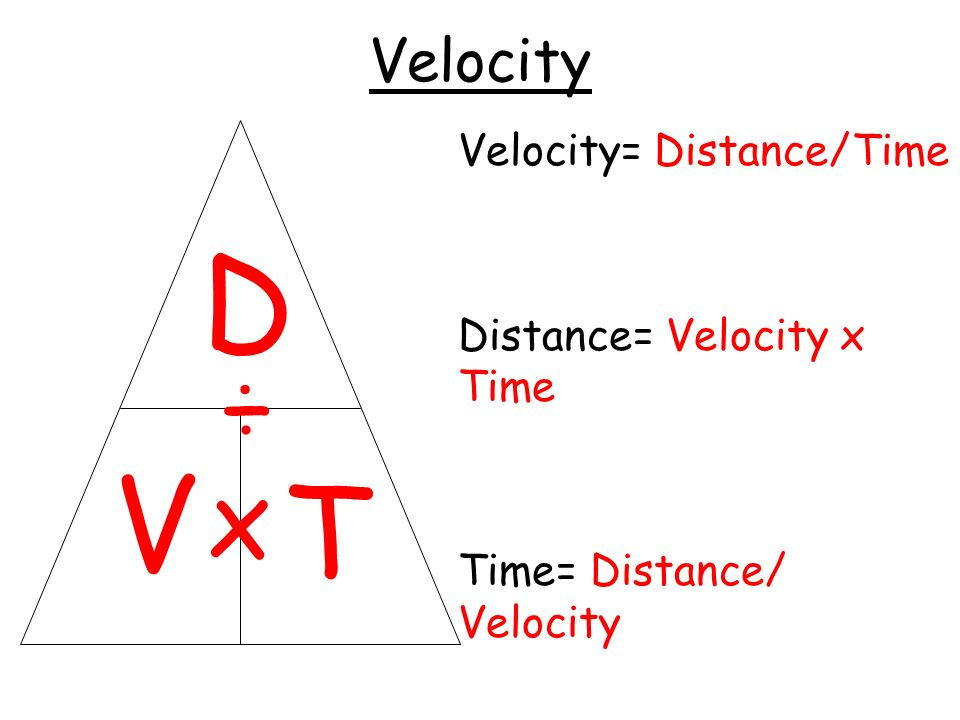
\includegraphics[scale=.3]{images/Velocity.jpeg}
    \caption{Diagram showing how to calculate velocity}
    \label{fig:velocity}
    \end{center}
\end{figure}

Momentum can be described as "mass in motion" every object has mass therefore if that object is moving it has momentum. Its momentum depends on the amount of mass that is moved and the speed that the mass is moving at.\\

\textbf{Momentum is calculated by using the formula:}

Momentum (P) = $Mass * Velocity$\\

Impulse is another factor that can change the power, speed and momentum of a boxers punch. When a punch is thrown and as it moves towards the head it has momentum while the head has momentum of zero. When the punch is connecting there is a transfer of momentum form arm to fist and then to the opponents head.

Depending on the opponent who your punch is connecting with damage can be decreased even by the slightest movement of his head this would increase the time interval meaning force of the punch is reduced.\cite{boxingPhysics}

\textbf{Impulse is calculated by using the formula:}

Impulse = $Force * Time$ \\

\subsection{Types of punches}
The degrees of angles and certain twists of the arm, fist is determined on the different kinds of punches.
\subsubsection{Jab}
Starting position hands near your nose with the fingers facing your chin.
As the punch is thrown extend your hand straight twist your knuckles so when the hand is extended fingertips are pointed at the ground.

\subsubsection{Hook}
Starting in a boxing stance, hands in the same starting position as the jab.
With the elbow at 90 degrees bring your forearm in front of you, finishing in the same line as your shoulders. The knuckles stay up with fingertips pointing at the ground.

\subsubsection{Upper Cut}
Starting position is the same a the Hook, boxing stance with hands near the nose. 
Your hand needs to swipe up from your hip while keeping elbow bent and fingers pointing towards your head. Imagining the punch finishing underneaths the opponents chin.\cite{punchingPhysics}


\subsection{Boxing Workouts}
Boxing is known as one of the most competitive, popular sports out there bringing athletes from all over the world to find out who is the most skilled has the biggest work rate and also who is the fittest.

\textbf{Cardio}\\
Endurance is one of the most important traits that a boxer can have. Boxing fight consists of 12 rounds and a boxer must have the ability to keep the highest fighting intensity during them rounds.
To get  a fighters endurance ready here are some simple exercises which even the most professional fighters use.
\textbf{Jump rope} this is a great exercise for endurance as the boxer is constantly moving both hands and feet. \textbf{high knees} and \textbf{heel taps} although these exercise seem harmless boxers cardio can be increased by executing theses exercises to the maximum intensity. \textbf{Burpee} this is a draining exercise used by top athletes its a very effective exercise improving endurance along with other muscles. \textbf{Shadow Boxing} and \textbf{Mountain climber} are exercises which help you to work on your breathing and technique while at the same time working on cardio.\\
It is recommended for beginners to start by executing each exercise for 1 minute and from then on keep adding on time or work without breaks in between exercises. \cite{cardioWorkout}.\\

\textbf{Gym}\\
Workouts in the gym can vary depending on what improvements a boxer needs, preparations for fights or just general conditioning.
For general conditioning gym sessions should be carried out 2-3 times a week exercises such as 
   \textbf{Squat (or leg press), Bench press (or chest press), Romanian deadlift, Crunch, Seated cable row, Triceps pushdown, Lat Pulldown, Overhead press, Biceps curl
 }.\\
If a boxer wants to work on specific needs such as power and strength the workout changes to suit the program.
The workout should be carried out 2-3 times a week including the following exercises \textbf{Romanian deadlift, Incline bench press, Hang power clean, Pull-ups, Squats, Combo crunches at 3 sets of 10 to 12
}.
\newpage
When fight preparations begin gym sessions should be changed to lighter loads and faster execution so the fighter can maintain their strength and power.
Workouts should be carried out 1-2 times a week containing the following exercises \textbf{Squats, Hang clean, Romanian deadlift, Crunches}.\cite{gymWorkout}\\

\textbf{Sparring}\\
Sparring in the ring is not about beating your opponent but its about making ring side improvements polishing on your technique and trying new things. Sparring is also about making mistakes its much better for fighters to figure out their mistakes in a sparring session than it the actual fight.  
Sparring is a great advantage for young fighters all of the top boxers out there practice sparring and have been sparring since a young age it gives young fighters the opportunity of gathering experience on top of learning from the best. 
Here are some of the learning outcomes from sparring with professionals.\cite{sparringWorkout}
\begin{itemize}
    \item Respect the opponents
    \item Everyone is at different levels of mindset and fitness
    \item It’s all about learning
    \item Don’t be too down if you’ve done badly
\end{itemize}

\subsubsection{Benefits}
There are many benefits of working out and exercising, boxing has the ability like any other sport to help people exit their realities.\\
Boxing workouts or any other workouts are known to reduce stress workouts boost endorphins,  moods, works as a form of meditation and its known to improves sleep, all of which aid in reducing stress.
Usually boxing workouts comprise of high intensity sessions with short recovery periods because these workouts are very demanding its not possible to think and worry about reality.\\

Workouts and exercises have many other benefits and advantages such as it improves cardiovascular health and decreases the chances of suffering from heart disease.\\

Keeping a consistent workout routine can help participants improve and gain total-body strength. Most if not all boxing workout consist of requiring the use of upper and lower body strength in their exercises while also boxing gyms incorporate other strength sessions within a workout. While it improves total-body strength it also enhances persons body composition which is the increase of muscle mass while decreasing your fat mass.\cite{workoutBenifits}   
\newpage
\section{Nutrition in Relation To sports}
 \textbf{Nutrition} is the study of how food and drink affect our bodies with special regard for the important nutrients required to sustain human health. It is a critical part of health and development. Nutrition is taken in to our bodies and used for growth, metabolism and repair.
\newline 
\subsection{Benefits of having a nutritious diet}
\begin{itemize}
    \item Good Nutrition Improves Well-Being 
    \item Helps You Manage A Healthy Weight
    \item Maintains Your Immune System
    \item Reduces The Risk of Chronic Disease
    \item Healthy Eating Positively Affects Your Mood
    \item Increases Focus
\newline    
\end{itemize}

\subsection{Nutrition for Athletes}
Food is important for athletes like boxers because it offers a great source of energy required for the action to be carried out. The food we choose to eat has an effect on our strength, training, performance and recovery.
Meals consumed before and after exercise are the most important in sports nutrition but you should really be careful with everything that you put into your body.
\cite{Nutrition}
\newpage
\subsection{Building and Repairing Muscle}
As well as good training to improve exercise performance, good nutritious diet is also important. Many athletes, especially those engaged in strength and power sports (boxers), eat a high protein diet believing this is necessary for muscle growth and repair, and the habitual protein intakes of some groups of athletes can reach values in excess of 2.5 g/kg body mass per d(5), with some individual values far higher than this.
\cite{maughan2012nutrition}
\newline
\subsection{Supplements}
According to an article from 2019, the rate of the intake of sports supplements was 82.2 percent, with the protein supplements being predominant (54.5 percent). Without further details, just by looking at this figure shows us that most athletes need supplements on top of their natural diet.
\cite{Supplements}
\newline
\subsection{Impact of Supplements}
Have you ever taken into consideration why athletes intake protein supplements?\\ Firstly supplements are usually taken either by powder or pills. Frequently powder supplements are taken with water, milk, juice etc... to make it taste better. Basically the intake of supplements are needed to create the amino acids that are needed to build muscle tissue, quicker and more efficiently. The reason athletes such as boxers benefit so much from the protein supplements intake is that intense physical activity demands higher protein levels than normal.
\\
\newpage
There are two types of supplements which  IOC and NCAA have ruled out. Some are allowed like the intake of protein powers, vitamins, amino acid etc.. But there are some which are prohibited and athletes could be fined quiet heavily or even a lifetime ban.According to the Department of Family Medicine, University of Tennessee College of Medicine–Chattanooga Unit, Chattanooga, Tennessee the following supplements are prohibited. \cite{jenkinson2008supplements}\\

\textbf{\emph{Anabolic steroids - Prohibited\\ Human growth hormone - Prohibited\\Ephedrine and pseudoephedrine - Prohibited\\Androstenedione and dehydroepiandrosterone - Prohibited}} 

\newpage
\section{Frameworks}

It was clear to us that the following frameworks, sdk's would be necessary to develop the application user friendly, ascetically pleasing and to give us the ability for the project to be developed on a work friendly platform.

\subsection{Angular}

\includegraphics[scale=.015]{images/angular.png}

Angular is a web application framework it's typescript based developed by an Angular team at Google.
It has been completely rewritten from the same team that built AngularJS.

Before we begin using Angular in our project we need to familiarize and rejuvenate ourselves with the following necessary languages \textbf{JavaScript}, \textbf{HTML} and \textbf{CSS} which are used in the framework.\\
The development environment must include both Node Js and npm package manager.\\
The latest Node JS version is 14.0.0 and the recommended version is 12.16.2. To determine the version of Node JS installed on your devices we simply type in \textbf{node -v} in the terminal.
The npm package manager is required for the downloading and installing of the npm packages.
\\To investigate if you have package manager installed you simply run the \textbf{npm -v} command in the terminal.\cite{angularSetup}

\subsubsection{Angular-CLI}
Angular CLI is a  command line interface that helps to simplify the development of high quality Angular applications. 
With angular CLI we are able to, develop, test, build, and deploy an Angular applications with very little trouble.
\newpage
\subsubsection{Meaningful commands}

This interface provides us with commands such as \textbf{ng new} this is used when you wish to create a new project, to produce code from already defined blueprints we run \textbf{ng generate} and \textbf{ng add} for adding framework support or application plugins necessary in the Angular project.

In the application we are able to run unit testing by executing the \textbf{ng test} command and for end to end testing we use \textbf{ng e2e}.

For compiling and running the application command \textbf{ng serve} is available this command runs the application locally on the web browser allowing us to view changes immediately.

\textbf{ng build} and \textbf{ng deploy} are used for building the application and deploying the build artifacts.\cite{angularGuide} 

\subsection{Ionic}

\includegraphics[scale=.1]{images/ionic.png}

Ionic is a complete open-source SDK for hybrid mobile app development created by Max Lynch, Ben Sperry, and Adam Bradley of Drifty Co.
Ionic is is an incredibly popular framework for many applications across many platforms it is known to be powering over 10\% of the Apple App store and 16\% of the Google Play store.\\
Ionic allows Web-developers IOS, Android and Web applications with one shared codebase. Using JavaScript, TypeScript and web API's it offers cutting edge web development experience.\\
Ionic consists of over 100 API integrations it has the capability to connect any Native API or SDK allowing developers to extend their applications to its optimum capacity.\cite{ionicInsight}\\

There are many advantages of using Ionic with developing an applications designed for a mobile platform it consists of an extensive amount of UI elements and quick prototyping. An Ionic UI component consist of two parts GUI and their functionality. It is available for the developer to change the way an element works, adding animations modifying, changing scrolling and many more adjustments are possible with ease.
\newpage
Other advantages come in to play as we progress into testing and building the application such as the simplified technique for the developer to test an Ionic application he does not require a testing device once The Ionic app works via webview the browser on the development machine can be used for testing.\\
Another massive advantage of using Ionic is the available documentation. Us as young developers we don't obtain a large amount of knowledge about ionic. Using an SDK with an in depth documentation could play a massive role in this project.
Ionics documentation is astonishing it covers an endless amount of useful topics explaining what these components are how they are used and how they connect.\cite{ionicPros} \newline

\textbf{User creates an application they have three options} 
\begin{itemize}
    \item Blank project with executing the following command: 
\begin{verbatim}
    ionic start myApp blank
\end{verbatim}
    \item Project designed with tabs by executing the following command:
\begin{verbatim}
    ionic start myApp tabs
\end{verbatim}
    \item Project designed with a side menu by executing the following command:
\begin{verbatim}
    ionic start myApp sidemenu
\end{verbatim}
\end{itemize}

\textbf{The application can be tested with the following command:}
\begin{verbatim}
    ionic serve
\end{verbatim}
This will deploy the application on your locally on your browser.\cite{ionicRun}
\newpage
\subsection{Cordova}
Apache Cordova is an open source framework that allows web developers to use their HTML, CSS, and JavaScript to develop a native application for mobile platforms such as IOS and Android.\\

Ionic and Cordova have been working very closely with each other since the very beginning of Ionic. Cordova has the ability to implement native mobile functionality and creating a fully native applications its biggest downfall is that it lacks a UI SDK.
With Ionic's components, navigation and platform specific styling Cordova working in conjunction with Ionic grants you the capability of developing a high performing native-like applications.\cite{cordovaInsight}

\subsection{Firebase} 

\includegraphics[scale=.05]{images/firebase.png}

This cloud application is designed by Google to help build. Firebase is a tool-set to “build, improve, and grow your app”, and the tools it gives you cover a large portion of the services that developers would normally have to build themselves, but don’t really want to build, because they’d rather be focusing on the app experience itself. This includes things like analytics, authentication, databases, configuration, file storage, push messaging, and the list goes on. The services are hosted in the cloud, and scale with little to no effort on the part of the developer.

This is different than traditional app development, which typically involves writing both front-end and back-end software. The front-end code just invokes API endpoints exposed by the back-end, and the back-end code actually does the work. However, with Firebase products, the traditional back-end is bypassed, putting the work into the client. Administrative access to each of these products is provided by the Firebase console.
\begin{figure}[h]
    \begin{center}
    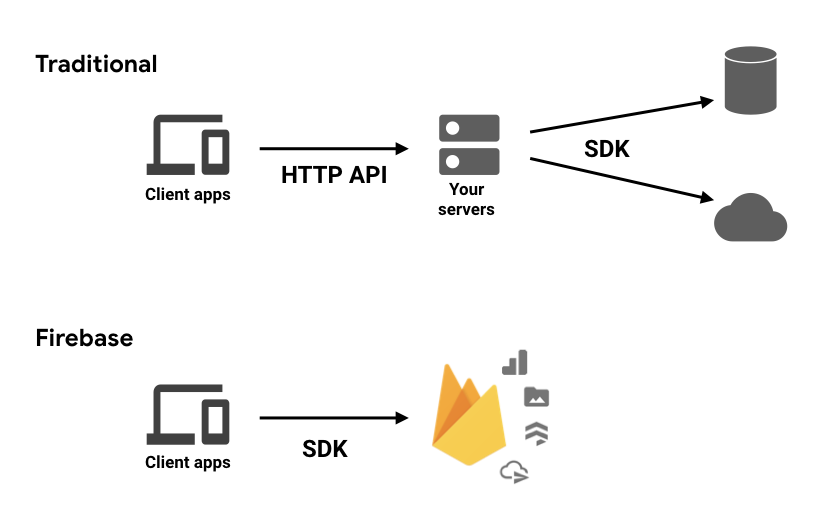
\includegraphics[scale=.5]{images/firebaseDiagram.png}
    \caption{Firebase console}
    \label{fig:firbase}
    \end{center}
\end{figure}
\newpage
\subsection{MYSQL}

\includegraphics[scale=.04]{images/mysql.png}

MySQL is a relational database management system based on SQL – Structured Query Language. The application is used for a wide range of purposes, including data warehousing, e-commerce, and logging applications. There are many versions of MySQL, we chose to use version 5.7.24.

In this project we use MySQL to store information about workout tips and meal plans. Users are able to view our seven day workout plan and meal plan through our homepage. The information is stored within the database and pulled when requested by user.
First we create the database locally through WampServer. WAMP is an acronym that stands for “Windows, Apache, MySQL, and PHP.” After creating and naming our database, we create a table within the database. 
This table is important as we need to pull information from this table. As you see this table has five columns. But the first column is unique, we are pulling information by the unique ID days. For example only workouts for Day-1 shall be printed out to the page that requests information about it.

\begin{figure}[h]
    \begin{center}
    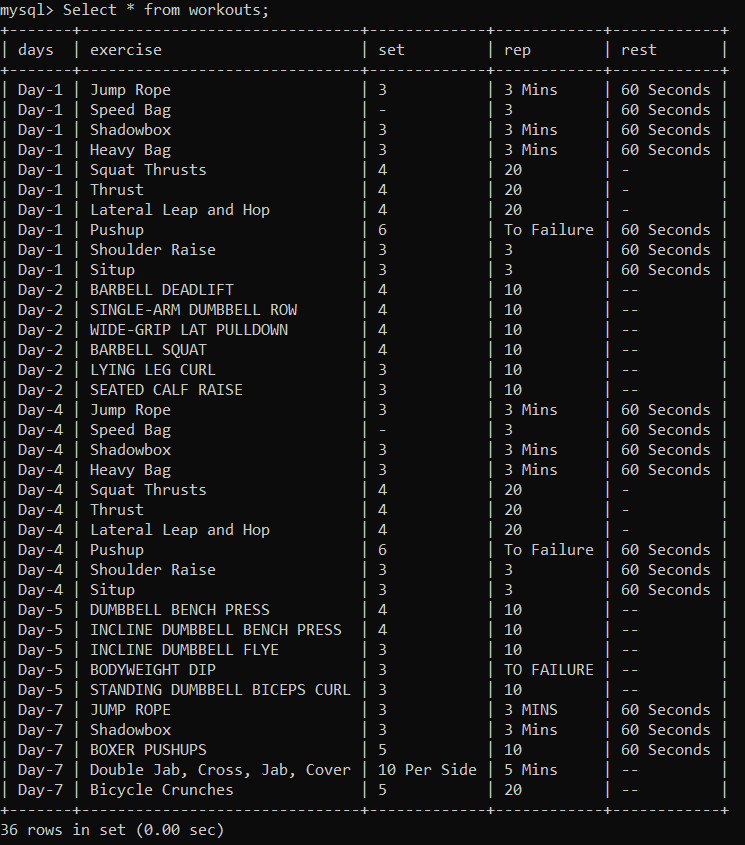
\includegraphics[scale=.56]{images/workouts-table.PNG}
    \caption{Workout excises in a sql database}
    \label{fig:MYSQL}
    \end{center}
\end{figure}

\subsubsection{How is this information displayed on web-page}
Within our project, we created a JavaScript file called "server.js". Within the JavaScript file we create a secure connection between the server and WAMP.
\begin{verbatim}
var connection = mysql.createConnection({
    host: 'localhost',
    user: 'root',
    password: '',
    database: 'workout'
});
\end{verbatim}
We are establishing a connection with our database above. Below we will show you how to pull information from AWS (Amazon Web Services). Basically, our database will be stored on a cloud where it will be available to everyone to view, whereas on the local machine only the creater of the database can view it now.

\subsection{Android}

\includegraphics[scale=.1]{images/android.png}

Android is a mobile device operating system developed mostly by Google. This was and still is the first reliable threat to the IPhone market.
\\
The Android working framework is based on an altered Linux kernel. The product contains Java applications running on a virtual machine. \\

Elements of the framework are written in Java, C, C++, and XML.
Google has partnered with multiple device providing organizations such as Samsung Htc and One Plus giving their clients options and variety that IPhone simply does not supply.\cite{butler2010android}\\

\subsubsection{Why Android Not IPhone}
The decision to deploy the application on android platform was determined by many advantages that android possesses over the iOS.\\
Since 2017 the number of android users is significantly higher than the IPhone users. Android has 64\% of the market share while IPhone has only 32\%.
Android users are double of the amount of IPhone users therefore if our application was created and designed for an android platform it would cover a wider market.\\

Another difference that helped us finalize our decision was the cost of publishing the application. Google Play has earned over \$ 3.3B in revenue while the App store made a huge revenue of \$ 5.4B. The iOS application store has produced a much higher revenue while possessing a substantially less amount of applications. Google play inherits around 2,800,000 available applications and the iOS platform consists of roughly 2,200,000.   
\\
The main reason that the revenue of iOS platform is much higher is due to the cost of publishing on the App Store.
\cite{android&iOS}

\begin{figure}[h]
    \begin{center}
    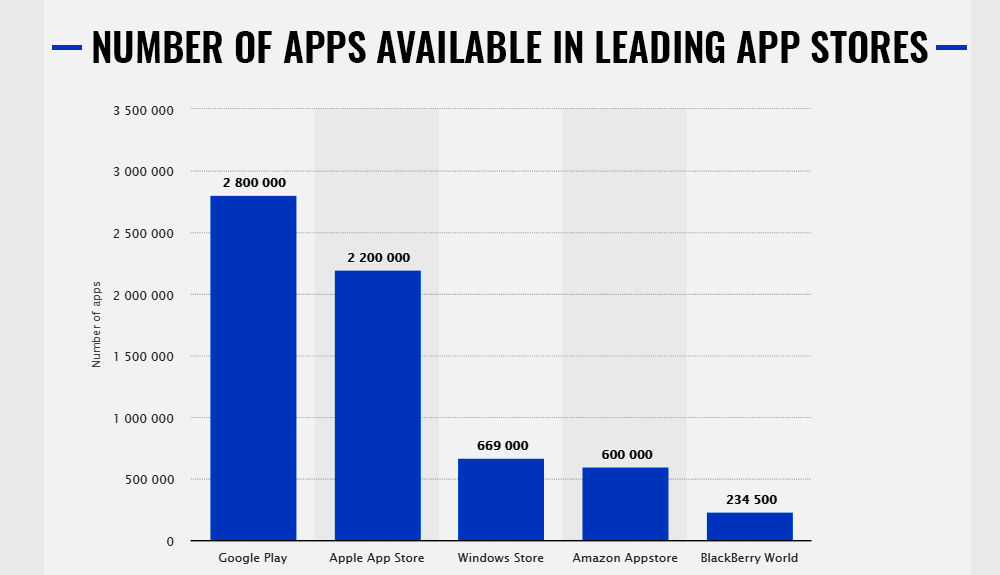
\includegraphics[scale=.5]{images/androidvsios.png}
    \caption{Chart showing the number of apps in different app stores}
    \label{fig:numberOfApp}
    \end{center}
\end{figure}

\subsubsection{Android Framework}

Creating the current software program we required a framework to develop and deploy an android application for the purpose of testing and customer use.\\

We had been slightly aware of Cordova through a previous module during our software course.
The agreement on Cordova came with no hesitations, using it presented us with the availability of deploying the application on Android, iOS and Windows. 
Cordova is a framework with many plugins that we had required for the completion of this project. 
It was clear that using Cordova would have a positive impact on our project, with the ability of testing applications on both platforms Android and iOS.
\cite{cordova}\\

Verdict on the application's platform was completed and our decision was made. We had agred that the application will be developed for both Android and iOS but will only be developed on google play for the android users. 

\section{Wearable Devices}
\vspace{5mm} %5mm vertical space
The availability and ownership of fitness devices and fitness applications has largely increased. Flurry an American mobile analytics, monetization, and advertising company founded in 2005 had completed a recent study on app users.
They have announced that the usage of health applications are growing 87 percent faster than the entire mobile industry.

One particular area of the mobile health market that is rapidly increasing are wearable devices. With Google Fit, Apple HealthKit, Samsung Gear and many other devices these accessories empower the customers in controlling, managing and tracking their fitness lives.\cite{rhodes2014accessing}\\

One of many objectives assigned to this project was to deploy the application on to wearable fitness device. 
For this to happen it was necessary for us to research and come up with reasonable options for a device and explore them in more details.

The option that we decide to use in the testing of our application must be able to determine users movements with sensors such as accelerometer also needs to be capable of receiving, collecting and sending data to a software program.\\

Options that we had came up with were 
\begin{itemize}
    \item Mobile Phone 
    \item Fit Bit
    \item Accelerometer chip
    \item Activity trackers
\end{itemize}

It was concluded that the application will be ran and tested on the phone at first when this is improved and upgraded we would move to connecting the application to a Fit bit or an accelerometer chip.

\subsection{Mobile Phones}
Mobile phones include endless sensors that we don't even realise exist with the modern technology.
Motion sensors such as the Accelerometer, Gyroscope and Pedometer sensors measure the movement of a human being. \\

The accelerometer sensors measure the change in the x, y and z axis. Gyroscope measures and detects each degree of changes in orientation. While the Pedometer is an advanced version of the accelerometer it is mostly used to track a persons steps accurately.\cite{sensorsPhone}   

\subsection{Fit Bits}

Fit bits like phones work with certain sensors. Most of the time fitbits use a three-axis accelerometer they can tell if you are moving forwards, backwards, side to side or even up and down.
By analyzing all the data recorded by the watch it can tell if you were walking, running, jumping or simply just moving your hands.\cite{sensorsFitbit}

\subsubsection{Ultimate goal}
We feel like the mobile phone device and the fitbit would suit the project for the moment but we don't believe that either one of them options would be reasonable for a boxer to wear or hold while training.\\

The ultimate goal of a wearable device for this application it would be necessary to design and develop hardware that could be inserted into a boxing glove and there would not be a worry of holding or wearing a device.
\newpage
\section{Survey}
\vspace{5mm} %5mm vertical space

We had designed the following application to be used in everyday life even by the most vulnerable, we understood that the application had to be effective but easy to use at the same time. Decisions on what was most substantial information to include in the application needed to be finalized.\\

As the designing and developing team of the application it was necessary that we could answer the following questions. \\

What are the main factors and reasons that make an application unusable and complex especially for people that lack in the knowledge of technology.

One of many reasons for applications not succeeding at present is determined by many factors. We decided to look more into certain factors which we defined as the most important to maximize the performance and simplicity while not damaging the performance or the aestheticism of the application. 
\cite{DesignFailure}\\

The factors that we believe are essential to making the application successful and we decided to look at in more detail were as follows

\begin{itemize}
    \item First Impression
    \item User Interface
    \item Target Audience
    \item Speedy/Performance
\end{itemize}

Today, most applications are dismissed by clients ultimately leading to their failure due to poor user experience.

An unsatisfactory result of the applications performance usually ends up with uninstalling it in no time. 
\cite{AppFailure}


Our decision to gain much more information was through out the form of communicating with the outside word. Our objectives from this was to gather opinions, ideas and possible improvements to the application.
We had created and deployed a survey to our class mates, relatives, friends and made it available throughout many social media platforms such as Snapchat, Facebook and Instagram. 
This in fact would help us to improve the knowledge of what people expect and would like to see in such application while also allowing us to elevate the quality and performance.\cite{surveyReasearch}

\subsection{Survey Questions}

\begin{enumerate}
    \item What is your gender ?
    \item What age are you ? 
    \item Do you own a sports/fitness device ?
    \item Do you use your sporting device while exercising ?
    \item Do you find your fitness device useful during or after workouts ?
    \item How many times do you exercise a week ?
    \item How important are statistics of a workout for you ?
    \item Do you rather follow already made plan or your own plan ?
    \item Are you aware with the reasons for each workout and what it improves ?
    \item If you could add a functionality to your application what would that be ?
\end{enumerate}
\newpage
\subsection{Survey Results}

After a few weeks of getting responses to the designed survey we received the results.
This survey was mostly completed 70.97 male and 29.03 percent females.
87.10\% of users were between the ages of 18-24 with 9.68\% over the age of 25 and finally 3.23\% under 18s.

We were presented with surprising results when asking if people own a sporing device in question three.
43.33\% of responses answered no while 56.67\% answered yes. We expected a much higher percentage in people owning a sporting device. We have come to the conclusion that participants didn't include their mobile devices as a sporting device therefore results didn't elevate as expected in this answer.\\ 

The result gave us insight that the if people use their devices while exercising where it stated that 10\% always use it 40\% sometimes and 30\% never use it.
We established if people find a fitness device useful in question five of the survey. Output of this question is very much divided 13.33\% of answers are both Extremely Usefully and Not Useful at all while majority of answers 46.67\% find it somewhat useful.

We needed to find out if people exercise often during a week to determine if this application would get enough attention from the user.
The result came back with a 53.34\% of respondents exercising three or more times a week while 6.67\% of responses came back as I don't exercise. 
This was a positive outcome because we believe that it would get enough use during the week by the user to get it tested and for it to become a permanent application on the users device.

It was important to verify if the users find statistics important, plans they follow and the reasons for certain workouts.
Only 3.33\% of people think statistics are not important while 30\% find them very important and 10\% extremely important.
Answers to question eight were very balance where people answered which plan they rather use plan already designed for users came out on top by a 10\% higher result.
We received the result for the second last question and we concluded that most people are aware of what each exercise is designed for. 53.33\% of responses were somewhat aware of reasons and improvements of each exercise.

The final question from the survey was on the improvements that people see on the already made applications.
We needed to to make a decision on what to add to the application this would be the first place we had to analyze.
The responses that we obtained were such as.
\begin{itemize}
    \item  Multiple plans available
    \item Heart rate monitor, breathing apparatus, step count
    \item Calories Burnt 
\end{itemize}
   
\subsection{Reflection on survey} 
This was a very important survey with a very successful feedback. The following results stated above helped us with the finalizing the design of the application.
It had supplied us with massive amount of ideas and possible solution. Its important to gain peoples feedback and apprehend their ideas. At the end of the day this application will be designed for everyday use by the mankind.

\begin{figure}[h]
    \begin{center}
    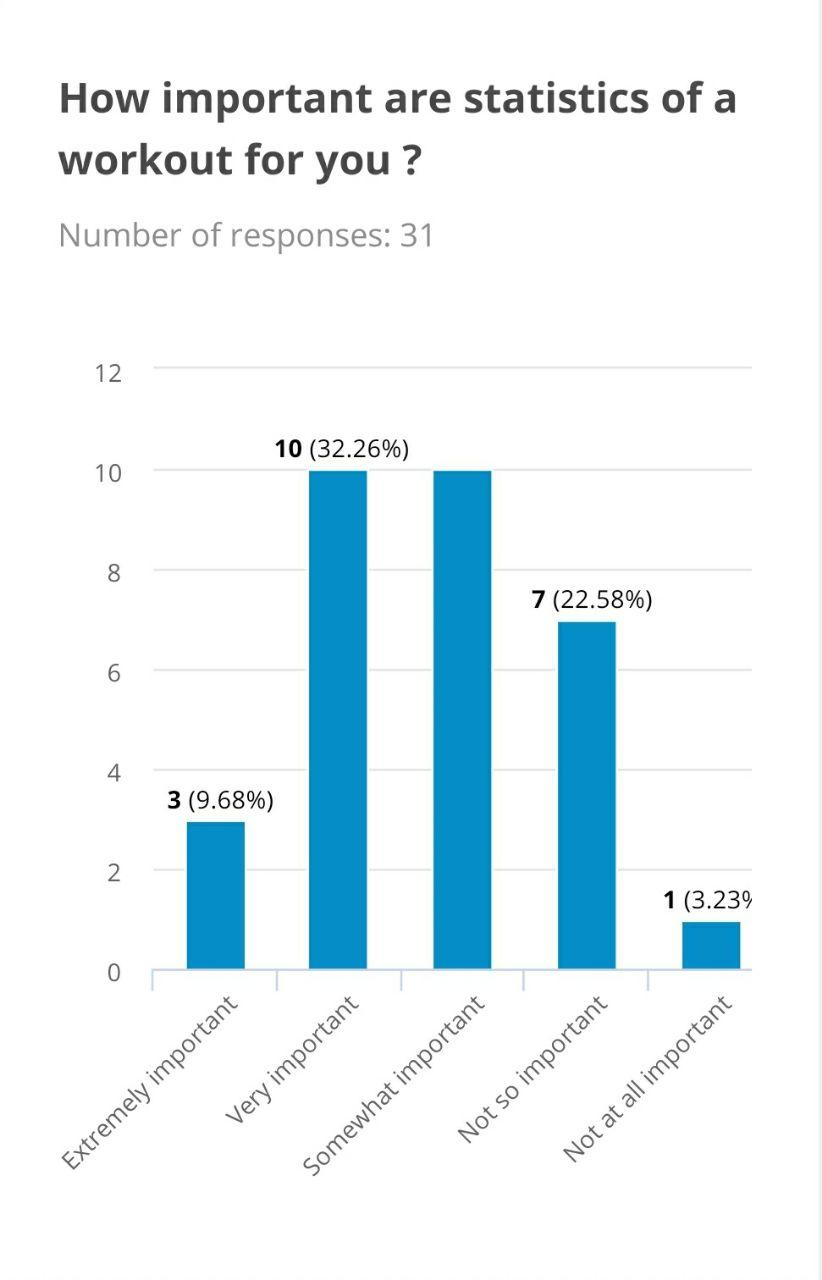
\includegraphics[scale=.2]{images/statistic1.png}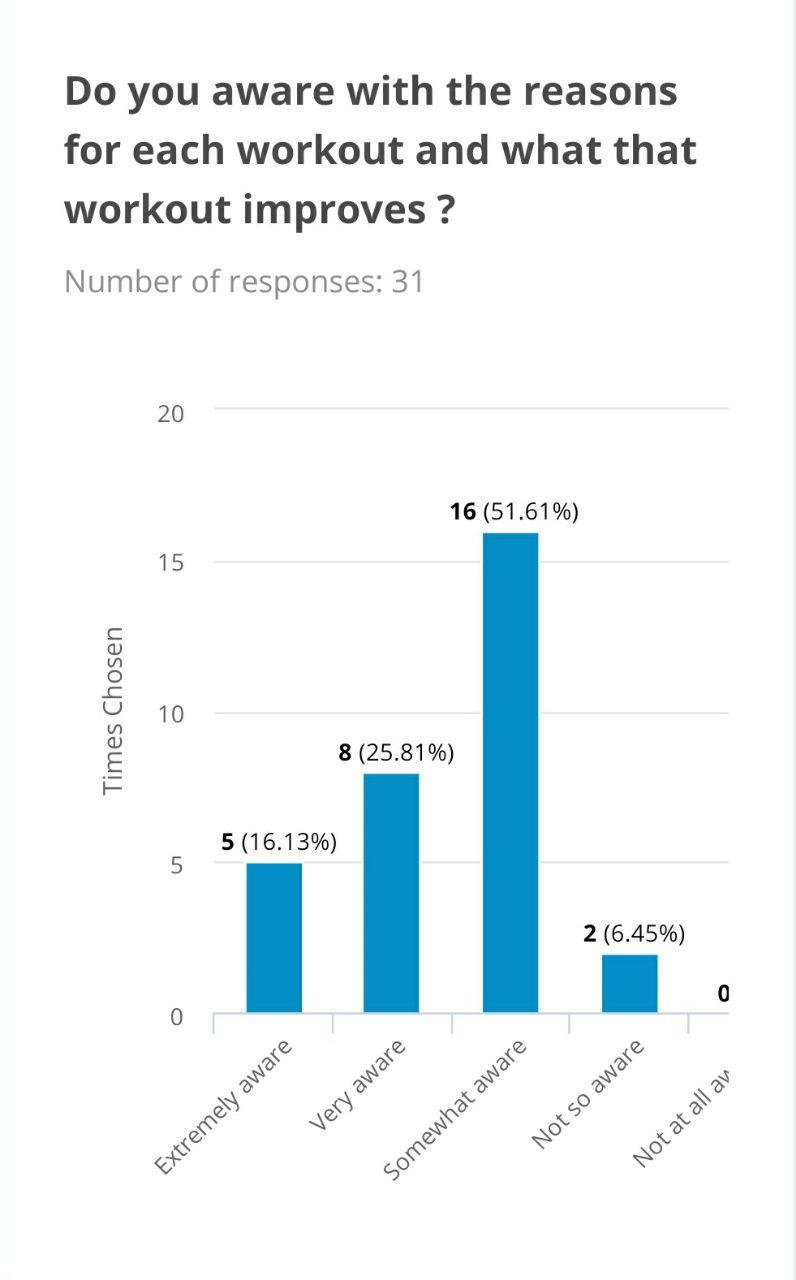
\includegraphics[scale=.2]{images/statistic2.png}
    \caption{Bar chart showing survey results}
    \label{fig:survey}
    \end{center}
\end{figure}

\newpage
\section{Artificial Neural Network}
In the oxford dictionary it says, “artificial intelligence is an area of study concerned with making computers copy intelligent human behaviour \cite{knowles2006oxford}.” If you google the question that I just asked, you’ll get something like “the theory and development of computer systems able to perform tasks normally requiring human intelligence, such as visual perception, speech recognition, decision-making, and translation between languages.”

To really understand what Artificial intelligence (AI) is, we first must know what Intelligence is. When people talk about intelligence, they identify it with “the ability to solve hard problems.” Some people say it’s “Maybe it is too early
to define intelligence. It is obvious that, after decades of study, we still do not know very much about it. There are more questions than answers \cite{wang2007logic}.” This is where we stumble upon the idea of Artificial Intelligence.

\subsection{Origin of the idea}
The birth of AI is bizarre from what normal people would think. AI was not made along with computers it was sort of this fictional monster. The first AI possibly made was by Mary Shelly when she wrote Frankenstein in 1818 \cite{shelley2012frankenstein}.So technically the first ever AI was made long before we even thought of the idea. The main concept that comes into people’s minds is something man made that is designed to solve all our lives biggest questions. \cite{bostrom2014ethics}

For this project we have to learn how to build a neural database. To build the actual neural network we are using a program called Keras which comes with Anaconda, a powerful tool used with Python. We look at different approaches when it comes to training a system. For example, taking this project in hand, we need to train the system to recognize the different types of punches thrown. Before learning out neural networks we would need to know what a neuron is.

\subsection{Neuron}
\textit{"A specialized cell transmitting nerve impulses; a nerve cell."} \\ A neuron has an input($x$) and output($y$). The input normally has a weight to it and a bias($b$) with is usually This image below will show you how a neuron looks.

\begin{figure}[h]
\begin{center}
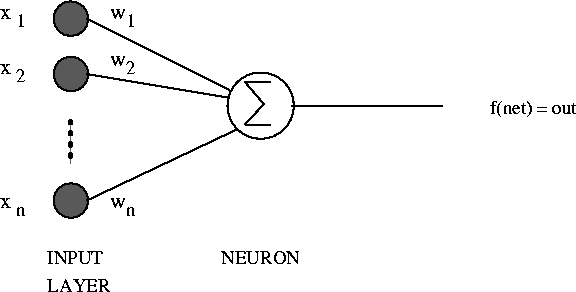
\includegraphics[scale=.4]{images/Neuron.png}
\caption{Diagram of Neuron}
\label{fig:neuron}
\end{center}
\end{figure}
Neural networks are a set of algorithms, modeled loosely after the human brain, that are designed to recognize patterns. Neural networks are being applied to many real-life problems today, including speech and image recognition, spam email filtering, finance, and medical diagnosis, to name a few.
\begin{figure}[h]
\begin{center}
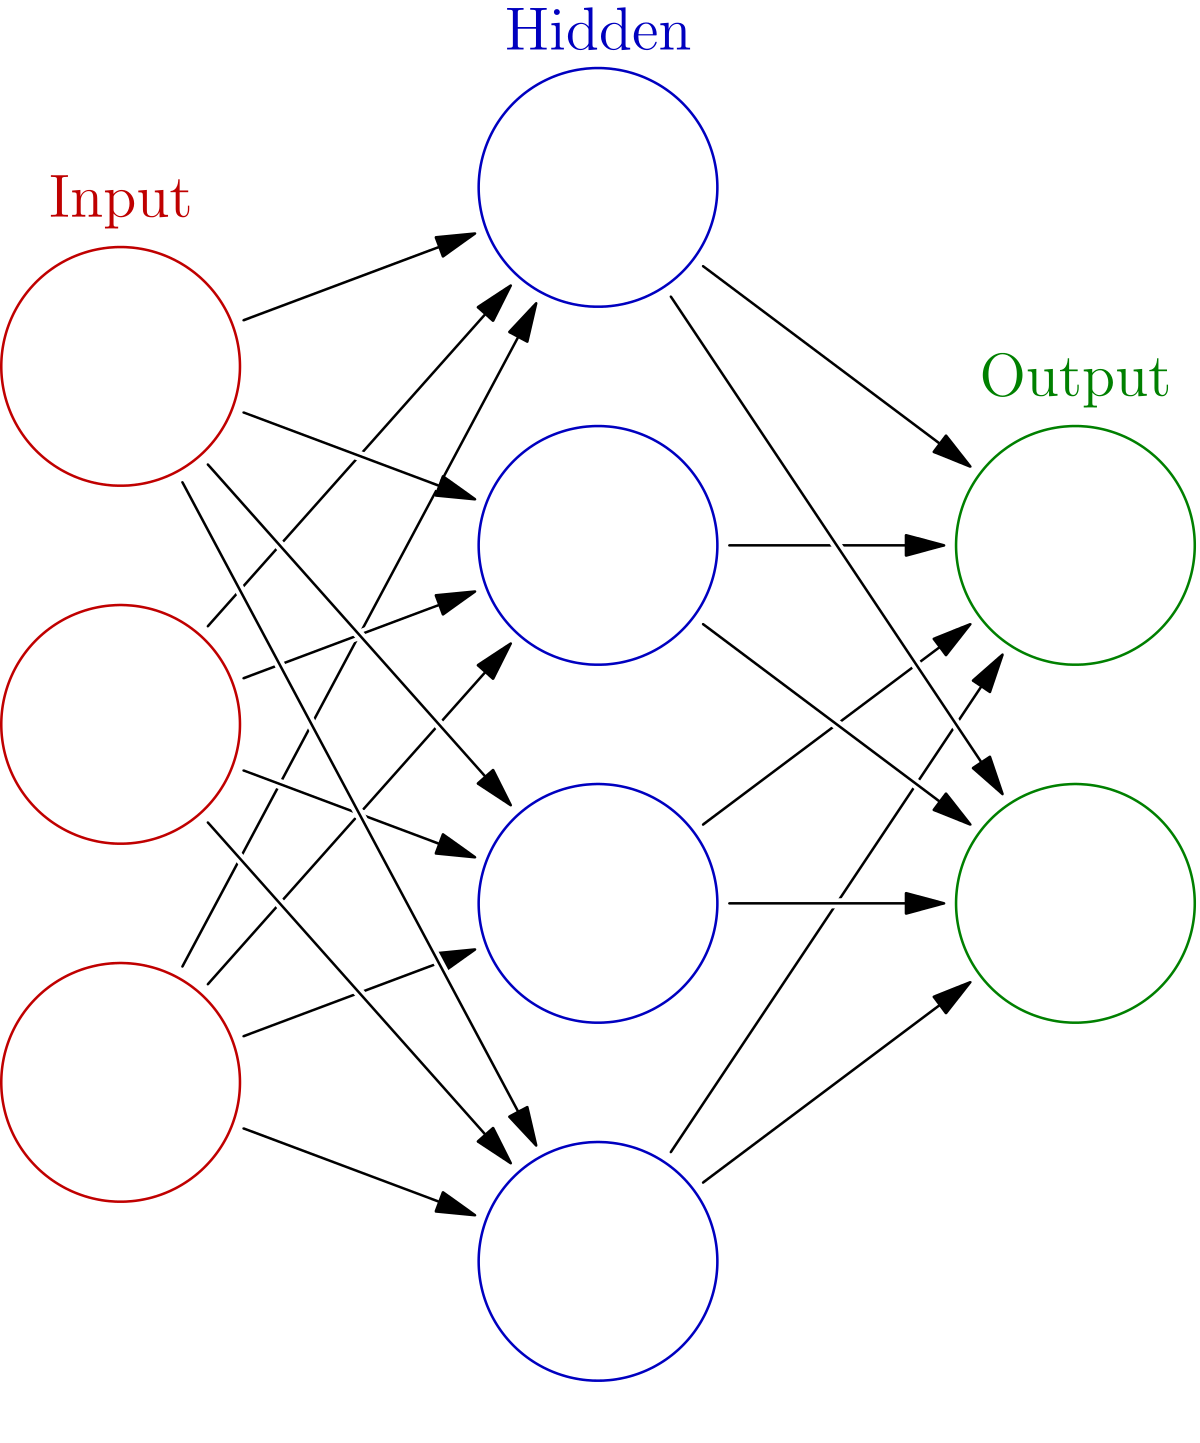
\includegraphics[scale=.18]{images/NeuralNetwork.png}
\caption{Diagram example of Neural Network}
\label{fig:NeuralNetwork}
\end{center}
\end{figure}
\subsubsection{3 reasons to study neural computation:}\\
\textbf{1.} To understand how the brain actually works: it's very large and very complicated and made from things that die when you poke it, so we need to use computer simulations.\\
\textbf{2.} To grasp a neuron-inspired model of parallel computation and their adaptive connections: it is a very different style from sequential computation.\\
\textbf{3.} To solve practical problems by using novel learning algorithms inspired by the brain: learning algorithms can be very useful even if they are not how the brain actually works.
\\
With these tools, we can train the model to recognize the type of punches:\\
\textit{Jab\\hook\\Uppercut}
\subsection{Tensorflow}

\includegraphics[scale=.04]{images/tensorflow.png}

Using Tensorflow with python to do this project. Tensorflow is a symbolic math library which can be used for machine learning. Keras is used to make the neural network. Numpy and pyplot is used to plot the data. This software allows developers to create a large-scale neural networks with many layers. This is used with python and has many uses in predictions and classification. Before making the data set for machine learning we'd need to learn of the core core concepts of making data-sets.\\This is how to shape your data and how to get it ready for training. To understand the layout of data-sets I used some examples online and decided to use the well know the iris data-set. This data-set collects data points from a hundred and fifty different samples of flower. It uses the petal length/width and the sepal length/width and sorts them into three types of iris.
\newpage
I wanted to do something similar to this using the x,y,z axis on the device and the accelerometer and sorting them into the three types of punches the device would register. I've learnt that by training a neural network with these values and telling it the type of punch it is I can then build a neural network than can reference from new values what type of punch is thrown. The data set that I'm going to make will contain four values and the type of punch it should be. The punch will be classified as 0, 1 or 2.
\newline
\begin{figure}[h]
\begin{verbatim}
from sklearn.datasets import load_iris

iris = load_iris()
iris

'data': array([[5.1, 3.5, 1.4, 0.2],
               [4.9, 3.0, 1.4, 0.2],
               [4.7, 3.2, 1.3, 0.2],
               [4.6, 3.1, 1.5, 0.2],
\end{verbatim}
\caption{Loading in the iris results into Tensorflow}
\label{fig:iris}
\end{figure}

\chapter{Methodology}

\section{Overview}
In this section we will describe and review the approach that we took in developing of this project, we will describe the methodology used why it was necessary, how it was implemented and how it helped the development of the application progress overall.
After reading this section the reader should have a clear understanding of the complexity and scale of the project as well as the steps taken throughout the development.
The project design was not fully completed and and features were not finalized therefore we needed to use a system that would help us keep on top of any changes and where issues could be dealt within an easy and efficient manner.
After researching many methodologies such as the Waterfall, Lean, Kanban we had decided that the best methodology for our project was Scrum which is an agile project management methodology or framework.
Agile methodology is a way of continuous iteration of both developing and testing. Unlike the Waterfall methodology which was an option for us to use both development and testing of the project are concurrent. 
There are many benefits of using this methodology and here are some of the ones that helped us determine that this was the right decision.
Agile allows the team to effectively prioritize features and workings also big changes to the project can be implemented even towards the end of the development.\cite{agileResearch}
\newpage
The agile methodology was a perfect way to help us with the development but we did were not able to utilize all of its features such as the daily scrum meetings we instead had a team meeting once a week discussing the work completed and forward approach. We attended meetings with our supervisors as often as possible informing them on the progress and gathering their thoughts on the progress as well as the necessary future development.   

\subsection{Using Scrum}
Scrum consists of six different stages.
\subsubsection{Product Backlog}
This is where the product owner builds a list of bright ideas and features that could possibly be developed into the project.
They then prioritise the list and bring the top items to the developing team.
\subsubsection{Sprint Planning}
The team, product owner and the scrum master discuss the top priority user stories and determine which ones will be implemented in the next sprint.
\subsubsection{Sprint Backlog}
Is the list of the user stories which are committed for the next sprint.
\subsubsection{Sprint}
This is a one to three week time frame where the user stories in the sprint backlog are developed by the team. During the sprint daily scrum occurs this is a team stand up meeting in which they discussing the completed work, the part each person is working on and if there are any blocked items or if anyone needs help with any part of their development.
\subsubsection{Potentially shippable Product}
After the sprint is completed the product owner decides if the project is ready to be shipped or if additional features need to be implemented.
\subsubsection{Sprint Review \& Sprint Retrospective}
Sprint review is where the team show the work developed on the project to the product owner and sprint retrospective is where they discuss what can be done to improve the process.\\
\textbf{This Workflow is repeated for each sprint carried out in the project}
\section{Sprint 1 - Application Idea}

\subsection{Work allocation}
We are allocating this project into three sections.\\
\textbf{First Step:}
Firstly we are going to start our research. We are going to deeply research in how this wearable device is going to work and what it takes to develop this new piece of technology. We need to understand what language is going to be used in constructing this. We need to know what sensors are required and how all data is going to be recorded.\\
\\
\textbf{Second Step:}
During the term our research is going to be a piece of document in how this wearable device can be achieved and possible drawing and animations of how it may work. But to back up our research, we need a physical piece that we can show and present. So we as a group decided to construct an application that is downloadable on mobile phone. This phone application is an alternative to the wearable device. The application is going to record the number of punches. The application is going to record and store data. For example is it going to store the number of punches under a certain amount of time.\\
\newpage
\textbf{Third Step:}
Whilst two members of the team are constructing the application. One person is going to specifically manage the database. They will have the responsibility to create the AWS account and link it up to the database. Overall, they are responsible for the whole database section of this project and to link it up to the application, that is works efficiently.

\subsubsection{Work Allocation - Usman Sattar}
For the development of the project, the following sections were assigned to Usman Sattar.\\
Firstly, he was in charge of the front-end design of the application in the functionality of the homepage, workouts page and meals page. Usman tried to make the application as user friendly as possible by making sure the creativity was at its most, while also keeping in mind that the application had to be simple and user friendly.

Secondly and most importantly, Usman was in charge of creating the workouts and meals database using MySQL using WAMP server, creation and deployment of AWS instance. It was quiet hard for Usman to approach a new topic and to learn how AWS operates, creating and managing the database through the usage of WAMP server.

Finally Usman ensured that the database was available to everyone and to enable this feature, the database has hosted to a cloud server using the Amazon Web Services.

In Conclusion, the responsibility of creating, hosting and managing the database using the following three elements were important: MySQL, WAMP and AWS. Implementing this feature within the Application through JavaScript, and designing the front-end view of the project was the main responsibilities given to Usman. There were many other tasks outside this element shared amongst us which for example includes the report.

\newpage
\subsubsection{Work Allocation - Sammar Tahir}
In the project Sammar took up the task of making a server/database for the users, adding a neural network and learning about app deployment to the app store.

He was in charge of back-end work for the users and syncing users information with the other developers tasks. One of the main things we wanted to focus on was having this application ready for deployment on android so Sammar had to make sure the the app was meeting the requirements as changes were made to the app. These requirements were security issues as well as system integrity.

The punches sometimes would not be able to accuracy record the punches and Sammar was in charge of making them work with higher accuracy, to achieve this Sammar had to make an neural network that would read in a data-set of points that are made by the punches and the neural network is told what the output should be.

Sammar made a database for users using Firebase, this was so the development on other components could be focused on for faster workflow. Sammar made sure that the users had an easier experience logging in or signing up to the app. The main goal here was to in courage users to sign up for the app which would then allow it to use it often since there is no hassle originally opening the app
\newpage
\subsubsection{Work Allocation - Arkadiusz Mamala}
For the development of the project the following sections were allocated to Arkadiusz Mamala.

He was in charge of the workout and  profile components.These components needed to be designed, developed and implemented into the application.
As well as working on theses components Arkadiusz added the Lazy Loading pattern into the angular project for efficient routing purposes.

The workout component consisted of creating the manual punch detecting system, a working timer designed for the user of the application to decide on the time of the workout, punches counting system which would count all the various punches and also a feedback form calculated on the completed workout displaying various statistics of the carried out session.
Working with various plugins to determine various different punches depending on the data coming in from these android plugins.\\

The profile component was designed to be simple for the user to use and to consist of important and relatable information.
Working with the calendar plugin this component consists of the users calendar events their start and end date. The users ability to create an event in their calendar was also enabled into this component.\\

Due to the ownership of an android device Arkadiusz was given the task of deploying and testing the application on the android platform. This consisted of working with the deployed apk files and checking if the various plugins are working correctly in the application on the android platform. \\

\textbf{Project Dissertation Allocation}\\
The project dissertation was completed with the three of us working together. We had tackled each section together simultaneously discussing various topics, layout and the content.
We feel that the write up was divided fairly and evenly. Each one of us working on comparable amounts of this document.


\subsection{Frameworks, Technologies \& Languages}
\subsubsection{Installing \& Running Angular}
We use the Node Package Manager to install Angular-CLI we execute the following command in the terminal on your machine 
\begin{verbatim}
npm install -g @angular/cli
\end{verbatim}
To check if the CLI has been correctly installed the following command is used to check
\begin{verbatim}
ng version
\end{verbatim}

\subsubsection{Installing \& Running Ionic }
Very much like Angular Ionic requires for Node JS to be present before the user has an option to install Ionic.
Once Node JS is available user can start the install using the terminal the developer needs to use the following command 
\begin{verbatim}
npm install -g @ionic/cli    
\end{verbatim}


\subsubsection{Installing \& Running Cordova }
To be able to install Cordova Node JS and Angular CLI must be present. To install Cordova the user simply needs to enter the following command in their terminal
\begin{verbatim}
npm install -g cordova
\end{verbatim}
To find out the version of cordova installed on the device enter 
\begin{verbatim}
cordova -v
\end{verbatim}
in the terminal.\cite{cordova}\\
\newpage
Before we can run the application on a device the developer must add the specific platform that is used in the testing the application you can do this by entering
\begin{verbatim}
ionic cordova platform add android/ios
\end{verbatim}
in their terminal.
After the platform is added, you can generate the required .apk file with the command 
\begin{verbatim}
ionic cordova build android
\end{verbatim}

Running the application on the specified device is done with the input of this command 
\begin{verbatim}
ionic cordova run android --device   
\end{verbatim} while having the device plugged into the machine developing the application. \cite{cordovaRun}


\subsection{GitHub Repository}
The GitHub repository containing the entire project can be found at:\\ 
https://github.com/ArekMamala/FinalYearProject\\
The following sections listed below outline the different components in the repository with a link to each part.

\subsubsection{README}\\
This part of the repository contains a simple introduction to the final year project brief explanation and a guide on how to download  install and run the application on a given device or environment.\\
https://github.com/ArekMamala/FinalYearProject/blob/master/README.md

\subsubsection{LaTex}\\
This section of the repository contains the latex project that we used for the write up of the development of the project dissertation. This section also contains a PDF file of the complete dissertation.\\  
https://github.com/ArekMamala/FinalYearProject/tree/master/LaTeX

\subsubsection{Final Year Project}\\
This section of the GitHub repository contains the Angular environment code used to design and develop the application with all the plugins and imports necessary for the environment to run the application.\\
\textbf{Link:} https://github.com/ArekMamala/FinalYearProject

\subsubsection{Releases}\\
The releases of the project is the build android applications as we progressed through making of the application. Each release differs from another. This section also contains the latest release of the application which is available to work on android devices.\\
\textbf{Link:} https://github.com/ArekMamala/FinalYearProject/releases


\section{Sprint 2 - Design & Research}
\subsection{Scope}
The following Sprint focused on studying our project materials, such as an acceptable environment that we could use, which languages we could use and whether there were any external libraries or tools that we could use to enhance the overall reach.
\subsection{Researching Application}
There were many types of research taken into consideration for this sprint. This ranged from articles from Google Scholar including articles from universities, stack overflow, videos, and information from genuine sources. We reviewed many books, articles and papers with the help of Google School and the GMIT library resource available through GMIT's website.
\newpage
\textbf{Environments}\\
With careful research, we decided to go with the development of an application through ionic with the usage of Visual Studio Code. Knowing some basic knowledge of ionic from our module from previous year, it made it easier to understand when conducting further research in relation to ionic. Visual Studio Code includes embedded Git and support for debugging, syntax highlighting, intelligent code completion, snippets and code refactoring.\\
\textbf{Plugins}
During the process of our application development, the following are the necessary plugins that are currently utilized within the program:

\begin{lstlisting}
cordova-plugin-calendar 5.1.5 "Calendar"
cordova-plugin-compat 1.2.0 "Compat"
cordova-plugin-device 2.0.2 "Device"
cordova-plugin-device-motion 2.0.1 "Device Motion"
cordova-plugin-device-orientation 2.0.1 "Device Orientation"
cordova-plugin-gyroscope 0.1.4 "Device Gyroscope"
cordova-plugin-ionic-webview 4.1.3 "cordova-plugin-ionic-webview"
cordova-plugin-screen-orientation 3.0.2 "Screen Orientation"
cordova-plugin-splashscreen 5.0.2 "Splashscreen"
cordova-plugin-statusbar 2.4.2 "StatusBar"
cordova-plugin-vibration 3.1.1 "Vibration"
cordova-plugin-whitelist 1.3.3 "Whitelist"
cordova-sqlite-storage 4.0.0 "Cordova sqlite storage plugin - cordova-sqlite-storage plugin version"
\end{lstlisting} 
\textbf{Platforms}
\\
We than researched and finalise the platforms used for this application. We determined to test on both Android and browser. We added in the ios platform in case we decided to implement it in the near future. To test out our application, we need the following:
\begin{lstlisting}
ionic cordova platform add android
ionic cordova platform add browser
ionic cordova platform add ios
\end{lstlisting}

\subsection{Designing Application}
While constructing this application as a team, we required to take some vital steps in designing it. Strong communication is important when it comes to any sort of team working exercise. In this section, we discuss on how we enhanced our application with the following implementations.
\newline
The team, product owner and the scrum master discuss the top priority user stories and determine which ones will be implemented within our application. During the stage of planning for the design of the application, we came up with some top features for the design.

\begin{itemize}
  \item Tabs View
  \item Counting Punches
  \item Showing The Type of Punches Thrown
  \item Workout and Meal Plans using MySQL/AWS
  \item Secure Login/Logout System Using Firebase
  \item Feedback Report
  \newline
\end{itemize}

Before these items were implemented to our application, we thought it was best to make sketches like an architecture of the project. This will give us a better overview of how the application functions.

\newpage
\section{Sprint 3 - Implementation \& development}
\subsection{Initial Setup}
We started with making a basic angular application while discussing what pages to do first. The languages we mainly wanted to use were JavaScript and typescript. Our main focus would be to make sure everyone was one the same level of coding before doing anything major. Angular and Ionic were had helpful documentation that we could easily grasp. For user storage we used Firebase to store basic user information. This was useful because we could work on our core pages without worrying to much about the user server issues. This make us develop faster than we normally planned on putting us ahead of scheduling. The efficiency gave us an opportunity to work on the hardware sensors on the phone, we had to do some maths to see how a punch would work using an accelerometer. This was the most complex step as it required us to learn some psychics about boxing, the method on this works can be found in our research. 

This is where we started to integrate what we have researched individually together. We used the Firebase services to sync with the information the users would need for working out and also to store the results from the accelerometer's inputs. This can be seen again whenever the user logs-in on any device connected to the internet. At this point in development we wanted to have our own management server that would not be on Firebase. This should be different from the clients and store information that we can update at anytime without effecting how the application itself runs. This means the users will be able to get workout updates or meal updates without us having to do a new application release. We also wanted our pages to load a bit quicker and wanted to stop the load times some of us would experience when testing the application.
\newpage
\subsection{Punch Detection}
For the manual punch detection the device motion and device orientation plugins are used to determine when a punch is thrown and what punch is thrown. 
For this system to be commenced the user needs to click on the start workout button at the bottom of the application.
This button runs many methods from the application including the startPosition method and the start method which both enable the plugins to start calculating the X, Y and Z values.

The following bit of code is responsible for starting up the device motion plugin.
Once the refreshing frequency is set and the device motion calls the watchAcceleration method we can begin to save the values into local variables which are refreshed with the set frequency.
\textbf{Obtaining X, Y and Z values from device motion}
\begin{verbatim} 
      // the refreshing frequency of the values 
      var option: DeviceMotionAccelerometerOptions = 
      {
        frequency: 170
      };
      this.id = this.deviceMotion.watchAcceleration(option)
      .subscribe((acc: DeviceMotionAccelerationData)=>
      {
        // setting the local X, Y and Z vaues to the 
        // accelerations X, Y and Z 
        this.x =  acc.x;
        this.y =  acc.y;
        this.z =  acc.z;   
\end{verbatim}

After this we carry out the logic behind calculating punches with the research completed on the different types of punches, the different techniques and the testing carried out for the X, Y and Z values under exercising these different hand movements our theory looks as the following in code.
\begin{verbatim}
    if ( (this.z >=-13  && this.z <=-7 ) || ((this.zStart - this.z >= 6) 
    && (this.yStart - this.y >= 8)) ) 
    {
    \\Jab is valid carry add to count and display it out to the user
    }
    else if (((this.y >=-1  && this.y <= 3) && ( this.x >=-12  && this.x <=-8 )
    ||((this.xStart - this.x <= 6) && (this.yStart - this.y >= 7 )))) 
    {
    \\Uppercut is valid carry add to count and display it out to the user
    }
\end{verbatim}
This is the main functionality of the manual punching detection system the logic to determine these punches and the way we managed to connect to the plugins to receive these values.

The way the neural networks works is that there are three points that used for the punches. X, Y and Z that are then stored and matched with what punch the user was supposed to throw. They are matched up and then the neural network starts to learn and predict what the punch should be and see how many times it gets it right. This is repeated till the network starts predicting more accurately  
\newpage
\subsection{Log In \& Sign Up Database}
For logging in and signing up the user will be using Firebase. Instead of allowing the user to enter an email and password we wanted them just to enter a username. We did not want to personally information we didn't need. To get around this we used @fitness to trick Firebase into thinking the username is an email address. This is the main line of code showing how a user signs up using the application this line below creates a user for Firebase.
\newline
\textbf{ Creating user}
\begin{verbatim}
const res = await this.afAuth.auth.createUserWithEmailAndPassword(username +
    '@fitness.com', inputPassword)
\end{verbatim}

This means when signing in we'd have to add the @fitness to the end of the username. 
\begin{verbatim}
// This is using firebase auth to check if logIn is correct
const res = await this.afAuth.auth.signInWithEmailAndPassword(data.username +
    '@fitness.com', data.password)
\end{verbatim}

We also have error handling in place for when the user enters the wrong username/password. After logging in successfully the user should be brought to the main homepage. The user should be able to look at basic information about themselves when logged in and are able to log out on the same page they used to log-in. We used cards to show and hide information the user instead of loading them to a different page. the cards are very useful for having everything already loaded onto one page so the user doesn't have to wait and navigate through different pages.
\newpage
\subsection{AWS server, Wamp \& MySQL}
In order for the user to access information regarding workouts and meal plans, the decision of implementing AWS server, Wamp and MySql was taken. We didn't want to hard code in the information, instead one person went ahead and took the responsibility to set up the database and the AWS account in order to manage the database from cloud server. In chapter four, figure 4.1, you will see a diagram with the implementation of the complete database in the ionic application.
\begin{verbatim}
app.get('/api/mealday1', function (req, res){
  weekday = 'Monday';
  sql = 'SELECT * FROM meals WHERE weekday = ' + connection.escape(weekday);
  connection.query(sql, function (error, results, fields) {
      if (error) throw error;
      console.log(results);
      res.json(results);
  });
})
\end{verbatim}
Above is a piece of code which prints out the meal plan for Monday.
Responds with all the information regarding 'Monday' when a GET request is made to the mealday1 page. We made the weekday into an unique ID. Although all the weekdays are in the same table with the database, but we access them by the days. For example we call all the information relating to 'Monday' to be printed out.
\\
\textbf{Establishing a connection with AWS}
\begin{verbatim}
var connection = mysql.createConnection({
  host: '18.206.137.252',
  user: 'admin',
  password: 'admin',
  database: 'asuboxing'
});
\end{verbatim}
As you see in the above section of the code snippet, we are successfully making a secure connection with the virtual machine using AWS. To access to the database, we go to phpmyadmin to create a user and password and grant all privileges. This is allow us from us local machines to access the database using the above IP address. 

\section{Sprint 4 - Testing \& Debugging}
\subsection{Unit Testing}
Unit testing is a level of software testing where individual units/ components of a software are tested. The purpose is to validate that each unit of the software performs as designed.\cite{unitTesting}
We applied unit testing in the early stages of development when it came to testing the workout section that is written in HTML, CSS and JavaScript using Visual Studio Code. Workout is the main objective of this application as it requires the user to hold the device and application determines the type of punch thrown according to the user movement.
\subsection{Integration Testing}
Integration Testing is a level of software testing where individual units are combined and tested as a group. The purpose of this level of testing is to expose faults in the interaction between integrated units. Test drivers and test stubs are used to assist in Integration Testing.\cite{integrationTesting}
Integration testing is applied when carrying out tests between the database which is created in WAMP server and AWS. They both work side by side when it comes to displaying information to the application. Another example of integration testing is Ionic, Angular and Cordova working together which brings an excellent result.
\newpage
\subsection{System Functionality Testing}
\textbf{Punch detection}\\
We decided before Tensorflow is implemented into the project we needed a manual detecting system as a precaution if Tensorflow was not finished in time. We had tested the X, Y and Z values using the accelerometer to observe the changes in values when the punch is thrown and conclude a theory that would be used in the development of the detecting system.
\begin{center}
    \textbf{JAB}
\end{center}{}
\begin{table}[h]
    \centering
    \begin{tabular}{||c c c c c c||} 
     \hline
     \textbf{Values Tested} & \textbf{Test 1} & \textbf{Test 2} & \textbf{Test 3} & \textbf{Test 4} & \textbf{Test 4} \\ [0.5ex] 
     \hline\hline
     X VALUE & 0 & 0 & 1 & 0 & 0\\ 
     \hline
     Y VALUE & 10 & 9 & 9 & 9 & 10\\  
     \hline
     Z VALUE & 0 & 0 & 0 & -2 & 2\\
     \hline
    \end{tabular}
    \caption{Values before the punch is thrown in a starting position.}
    \label{tab:jabBeforet}
\end{table}

\begin{table}[h]
    \centering
    \begin{tabular}{||c c c c c c||} 
     \hline
     \textbf{Values Tested} & \textbf{Test 1} & \textbf{Test 2} & \textbf{Test 3} & \textbf{Test 4} & \textbf{Test 4} \\ [0.5ex] 
     \hline\hline
     X VALUE & 0 & 1 & 2 & 3 & 0\\ 
     \hline
     Y VALUE & 0 & 1 & 1 & 2 & 2\\  
     \hline
     Z VALUE & -9 & -9 & -9 & -8 & -10\\
     \hline
    \end{tabular}
    \caption{Values at the end of the punching process.}
    \label{tab:jabAfter}
\end{table}

As we can see above in figure \ref{tab:jabBeforet} are the values in boxing ready position and  figure \ref{tab:jabAfter} are the values at the concluding position.
The following conclusion from the above data can be drawn 
\begin{itemize}
    \item The X value usually stays in and around its initial value.
    \item The Y value decreases by an average value of 8.2.
    \item The Z value as well as the Y value decreases by an average value of 8.2.
\end{itemize}
\newpage
\begin{verbatim}
\\ Possible If statment Theory
    if((YStart - YEnd >= 6) && (ZStart - ZEnd >= 8)){
        Punch++
        Jab++
    }
\end{verbatim}


\begin{center}
    \textbf{UPPERCUT}
\end{center}{}
\begin{table}[h]
    \centering
    \begin{tabular}{||c c c c c c||} 
     \hline
     \textbf{Values Tested} & \textbf{Test 1} & \textbf{Test 2} & \textbf{Test 3} & \textbf{Test 4} & \textbf{Test 4} \\ [0.5ex] 
     \hline\hline
     X VALUE & 0 & -1 & 1 & 0 & -2\\ 
     \hline
     Y VALUE & 10 & 9 & 9 & 9 & 9\\  
     \hline
     Z VALUE & 0 & 2 & -2 & -2 & 0\\
     \hline
    \end{tabular}
    \caption{Values before the punch is thrown in a starting position.}
    \label{tab:uppercutBeforet}
\end{table}

\begin{table}[h]
    \centering
    \begin{tabular}{||c c c c c c||} 
     \hline
     \textbf{Values Tested} & \textbf{Test 1} & \textbf{Test 2} & \textbf{Test 3} & \textbf{Test 4} & \textbf{Test 4} \\ [0.5ex] 
     \hline\hline
     X VALUE & -9 & -9 & -9 & -10 & -9\\ 
     \hline
     Y VALUE & 0 & 0 & 0 & 0 & 0\\  
     \hline
     Z VALUE & 2 & 3 & 3 & 2 & -3\\
     \hline
    \end{tabular}
    \caption{Values at the end of the punching process.}
    \label{tab:vAfter}
\end{table}

As we can see above in figure \ref{tab:uppercutBeforet} are the values in boxing ready position and  figure \ref{tab:uppercutBeforet} are the values at the concluding position.
The following conclusion from the above data can be drawn 
\begin{itemize}
    \item The X value decreases by an average value of 8.8.
    \item The Y value decreases by an average value of 9.2.
    \item The Z value has on average a 3.1 increase.
\end{itemize}
\begin{verbatim}
\\ Possible If statment Theory
    if((XStart - XEnd <= -8) && (YStart - YEnd >= 9)){
        Punch++
        Uppercut++
    }
\end{verbatim}

\textbf{Log In Sign Up Database}\\
Most of the error handling is done within Firebase. As developers we have to enter the code that calls these functions to testing in our code. 

\begin{table}[h]
    \centering
    \begin{tabular}{||c c c||} 
     \hline
     \textbf{Test} & \textbf{Expected Output} & \textbf{Pass/Fail} \\ [0.5ex] 
     \hline\hline
     Creating new user & New user is created & Pass \\ 
     \hline
     Logging in with username/password & Log-In successful & Pass \\  
     \hline
     Logging out & Log-Out successful & Pass \\
     \hline
     Creating a user when an existing username & Username taken & Pass \\
     \hline
     Entering incorrect username/password & Log-In unsuccessful & Pass \\
     \hline
    \end{tabular}
    \caption{Test Case for Log-In/Sign-Up}
    \label{tab:LogInTest}
\end{table}

\textbf{Workouts Meals Database}\\
As a developers point of view, below are some test cases carried out in relation to the development of the database using MySQL, WAMP Server and AWS instance on cloud server.

\begin{table}[h]
    \centering
    \begin{tabular}{||c c c||} 
     \hline
     \textbf{Test} & \textbf{Expected Output} & \textbf{Pass/Fail} \\ [0.5ex] 
     \hline\hline
     Accessing database on cloud  & Database displayed & Pass \\ 
     \hline
     Logging in with username/password & Log-In successful & Pass \\  
     \hline
     Information Within tables & tables polluted with information & Pass \\
     \hline
     Deleting information from tables & Developers are able to add and delete  & Pass \\
     \hline
     Logging in via IP address & Access to AWS instance & Pass \\
     \hline
     Drop tables & Tables within database deleted & Pass \\
     \hline
    \end{tabular}
    \caption{Test Case for Log-In/Sign-Up}
    \label{tab:LogInTest}
\end{table}

\subsection{Acceptance Testing}
Acceptance testing is a software test level in which an acceptability test is performed on a system. The aim of this test is to determine compliance with the business specifications of the program and to decide whether it is appropriate for delivery. Once the entire application testing process was completed by the three of us, we decided to get a group of young athletes particularly focusing on boxers to test out this application for its acceptability. ASU Boxing application should have a flawless result in terms of meeting our expectation and what it is designed for.

\section{Sprint 5 - Deploying}
\subsection{Android Deployment}
We decided to android for developing our application. We choose android because the ease of use and developing. Android is one of many mobile operating systems based on the Linux kernel. Android was announced in Sept 2008 and has now become one of the most popular mobile operating system. Developing an app for android is simple using android studio and ionic. This is why we also choose ionic for our application. 

To deploy an app in the play store we'd need to
\textbf{Understand the Developer Program}, this can be found at:\\ https://play.google.com/about/developer-content-policy/
\subsection{App Store Deployment}
Following these guidelines we keep us in good standing with google play store and most importantly keep our users safe and protected. An example of this would be, our app should only request permissions that are only used for core features of the app while keeping clear of what personal data we use. To test against the quality guidelines:\\ https://developer.android.com/docs/quality-guidelines .The tests found here are the tests we are going to base our tests on. Example of these test can be found at \ref{tab:SecurityTest}.


\begin{table}[h]
\begin{tabular}{||c c c||} 
 \hline
 \textbf{ID} & \textbf{Description} & \textbf{Tests} \\ [0.5ex] 
 \hline\hline
 SC-D1 & All private data is stored in the app's internal storage. & SC-1 \\ 
 \hline
 SC-D2 & All data from external storage is verified before being accessed. & SC-2 \\  
 \hline
 SC-D3 & All intents and broadcasts follow secure best practices. & SC-10 \\
 \hline
 SC-D4 & No personal or sensitive user data is logged to the system or app-specific log. & SC-10 \\
 \hline
\end{tabular}
\caption{Data Security Testing google standards}
\label{tab:SecurityTest}
\end{table}


\chapter{System Design}
This is where you’ll find all the the designs that we did before starting the project. We needed to have a clear understanding of different levels of the application and the outline of the user UI before we started the coding process.

\section{Project Design}
\begin{figure}[h]
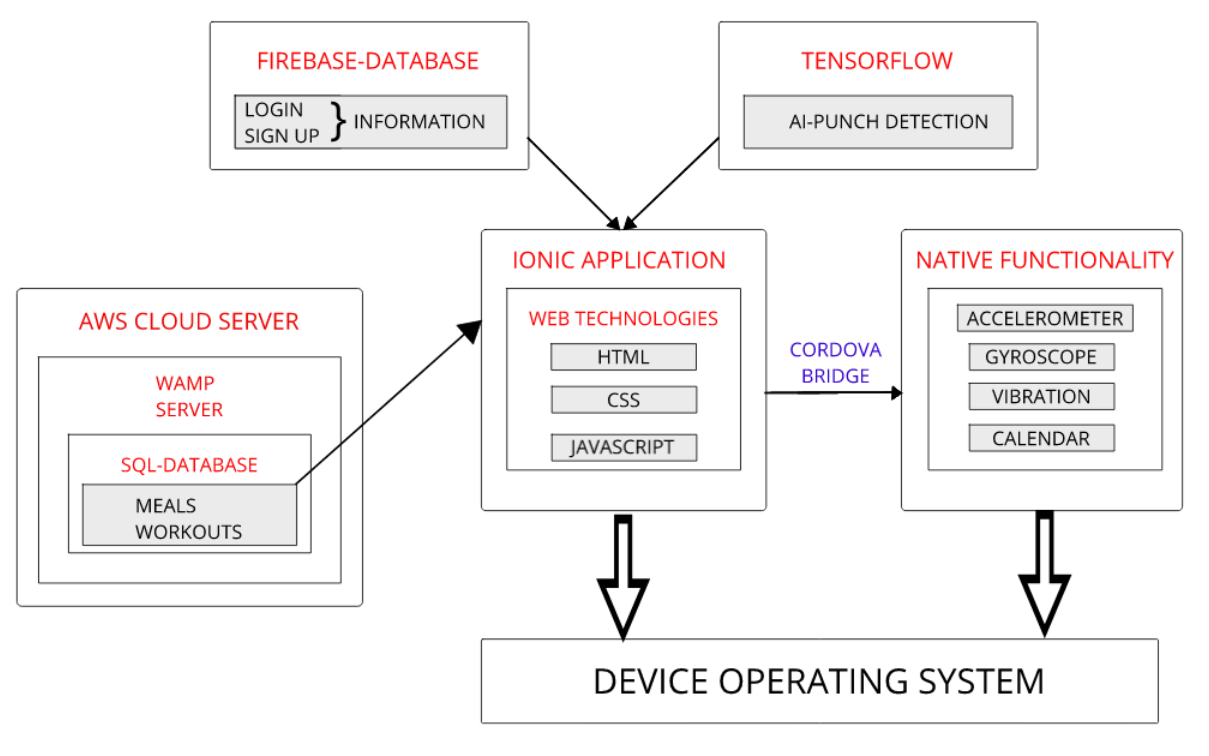
\includegraphics[scale=.37]{images/projectOverview.png}
\caption{Project architecture block diagram}
\label{fig:projectDiagram}
\end{figure}

Above image is the overall design of the entire project. We have an application working together with two databases one on the Wamp Server based on the AWS Cloud server and an online database for the users login and sign up information.\\
The design shows Tensorflow connecting to the ionic application for the AI punching detection system.\\
The application applying native functionality using Cordova getting deployed to the device operating system e.g. Mobile Phone. 
\section{Application Design}
This is the application design which describes the components that are included and the pattern that we decided to use in the project.
We finalized the decision of developing the application using the Lazy Loading pattern. This pattern is used for large scale Angular projects.
Since the application has databases, AI and servers working in line with it this pattern would be the best way increase our applications performance.
Below image is the application designed in the lazy loading pattern.
\subsection{Lazy Loading}
\begin{figure}[h]
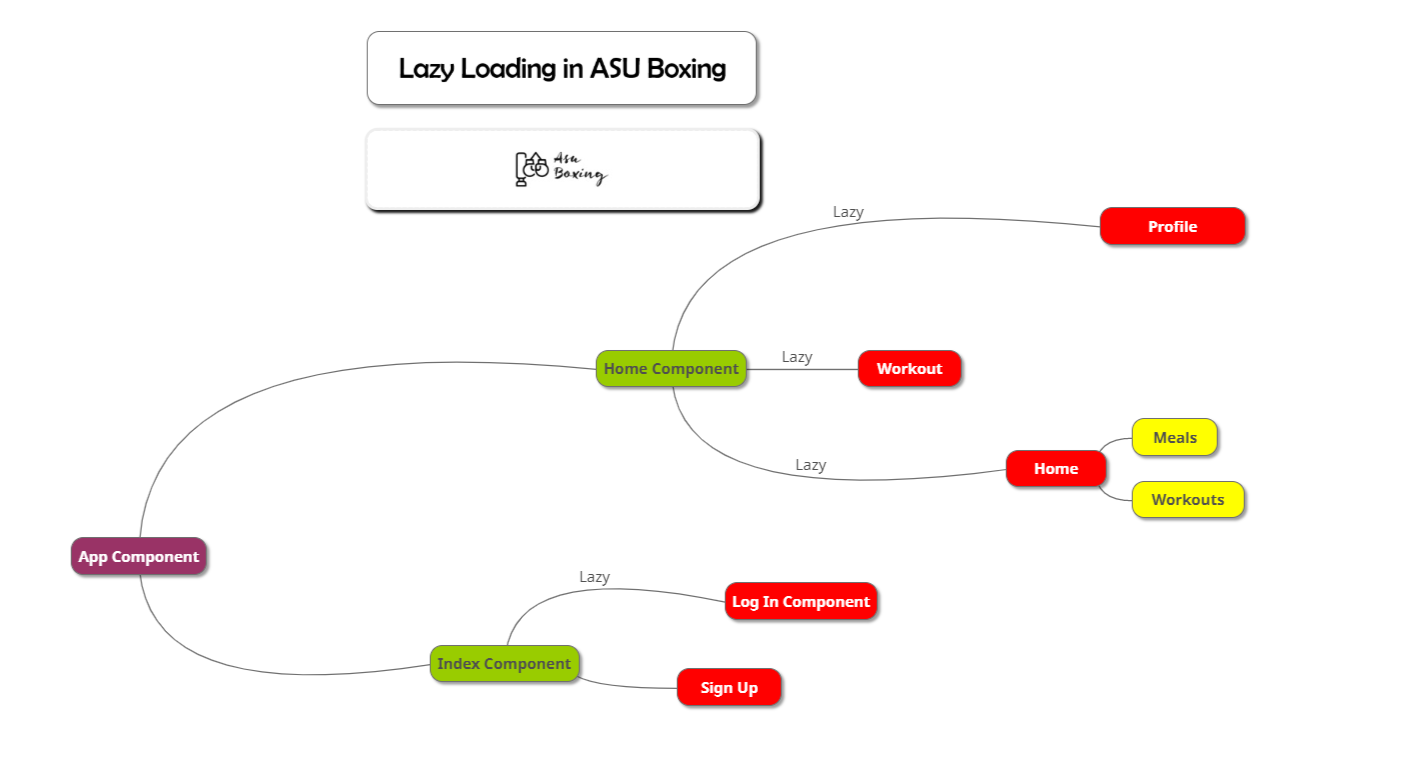
\includegraphics[scale=.5]{images/Lazy-Loading(4).PNG}
\caption{Lazy loading diagram}
\label{fig:LazyLoading}
\end{figure}
\newpage
As you can see in the above design app component is divided into two different components the Home Component and Index Component.
The main idea of lazy loading is for the project to load only the components that are necessary at the time of use. \\
Our index components is in charge of both the Login and Sign up parts of the application.\\
While the Home Component loads the Workout, Profile and Home products of the application which then load only the selected component depending on which product, Workout, Profile and Home components are available to be loaded. 

\section{Log In \& Sign Up}
The Log-in/Sign-up page should be very straight forward for the user to use. We decide that we should keep the page simple so users will more than likely sign up for the app. We didn't want them to share their email with us because we know some people don't like giving their user information away, instead we said they can just use their username and a password.

\begin{figure}[h]
\begin{center}
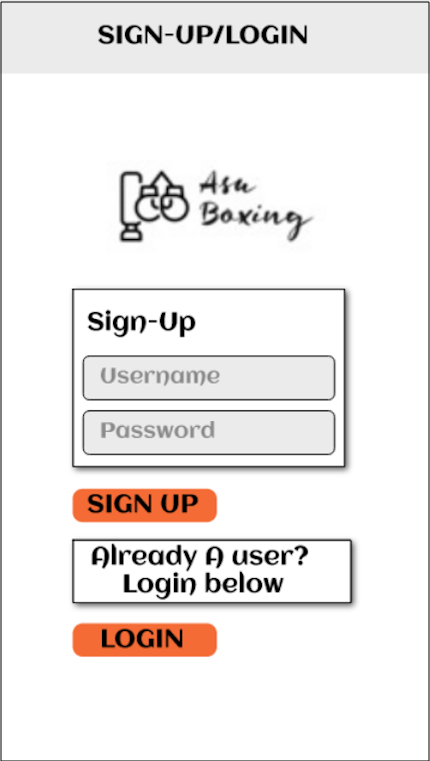
\includegraphics[scale=.5]{images/loginPageBorder.png}
\end{center}
\caption{Login page}
\label{fig:LazyLoading}
\end{figure}

Having the sign-up feature next to the log-in made it easier to get more users to make an account to store their personal information. From what they choose, we can store and load custom workouts which are unique for every user. 
\subsection{Firebase Design}
For storing passwords, we didn't want to have the passwords available locally. This is where Firebase base comes in. It encrypts the password for us and stores it so we won't be able to know the users passwords either. The safety of users information is very important in this day and age. We all agreed it would be best if we did not have access to the passwords and if any issues occurred the users could contact us and we can send a link for the users to reset their passwords. Shown in figure \ref{fig:firbase} we can see how Firebase handles most of the back-end server maintenance.

\section{Home Component}
\begin{wrapfigure}{R}{0.3\textwidth}
\centering
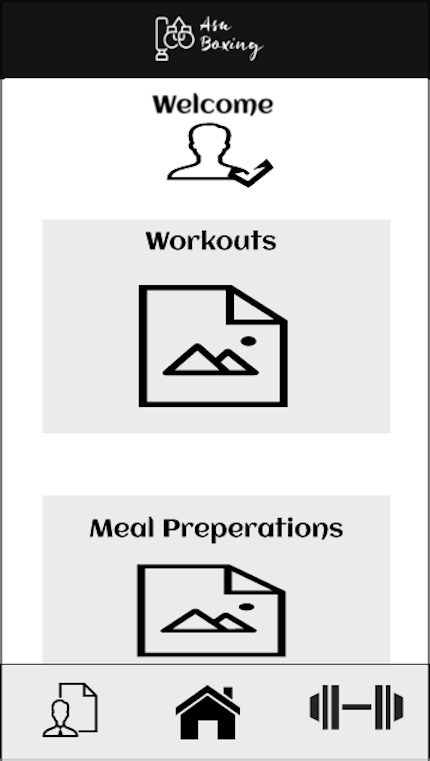
\includegraphics[width=0.25\textwidth]{images/homePageBorder.png}
\caption{\label{fig:homepage}Home}
\end{wrapfigure}
The main homepage is designed to be as simple and elegant with user friendly features. The homepage starts of with a simple slider where the user can slide through three images.
Further below we have the clickable ion-card feature for workouts which brings the user to our workouts page for their 7-day workout plan. Just to break up the page a little, we provide a motivational quote by Winston Churchill. Below that we have another ion-card feature for meals which is also a clickable feature that brings the user to the meals page for meal plan advisory.
\\
\newpage
\subsection{Workouts and Meals}
\begin{wrapfigure}{L}{0.3\textwidth}
\centering
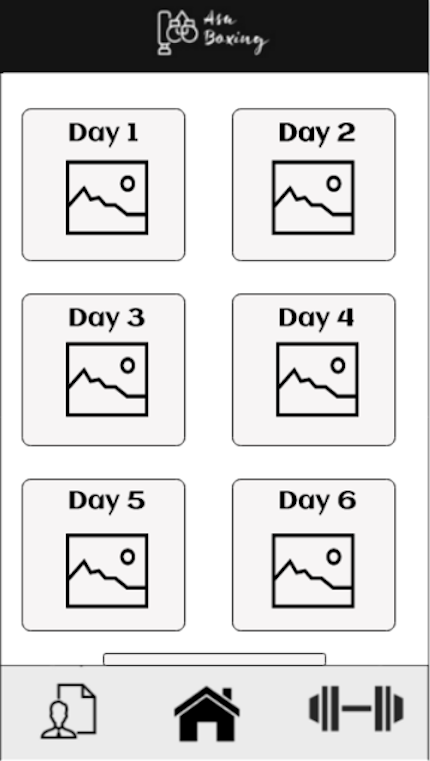
\includegraphics[width=0.25\textwidth]{images/days.png}
\caption{\label{fig:homepage}Dashboard}
\end{wrapfigure}
Both the meals and workouts page have the similar layout. These pages are designed using ion-cards. The ion-card features image and text in a card like look. For seven days, we create seven separate clickable cards which brings the user to another page which will be described below. It makes it simple for users to understand and navigate back and forth. As seen below in figure 4.6, once the user clicks on one the seven days, it will look somewhat like that in terms of design.\\\\\\\
\subsection{Workouts}
\begin{wrapfigure}{R}{0.3\textwidth}
\centering
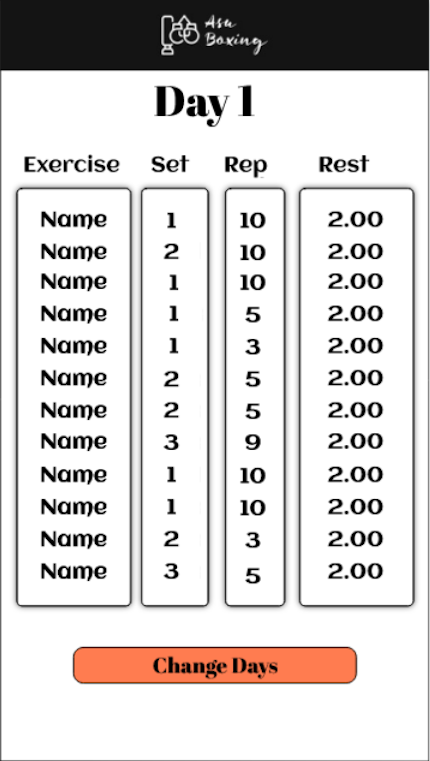
\includegraphics[width=0.25\textwidth]{images/dayWorkouts.png}
\caption{\label{fig:homepage}Days}
\end{wrapfigure}
This is an example of one of the workouts page. This is one way we can format the information from the database to the page. The information is extracted from a cloud hosted database using the combination of MySQL, WAMP and AWS. The information is extracted on the base of the days as the days are set to a unique ID. As seen in the image, there is an ion-button that brings the user back to the workouts dashboard where he/she can choose a different day to view.
For storing information regarding meals and workouts, we didn’t want to have the information available locally. This is where MySQL, WAMP and AWS comes in. It makes sense that the user can get to this information from anywhere and anytime by us linking the data through an IP address.

\newpage
\section{Profile Component}
We have designed the Profile component as a planner for the user to stick by and follow strictly.
For this to become possible the idea of a built in planner in the application was crossed out.
We wanted to use the ideology of "work smarter not harder" we decided to use the already available calendar application on every mobile phone.\\
This feature is designed to eliminate of the following scenario happening for example when a consumer decides to use the application and make plan for the following days, typically this would be saved in the application and only notify the user when accessing that application. This scenario can cause a problem for the user completing workouts as he/she can easily forget about their plans and not open the application in time to follow up on their programs.
By using the calendar application users will be notified that the workout is due even without accessing the application this will remind them to complete the workout and keep up with their program.

\begin{wrapfigure}{L}{0.3\textwidth}
\centering
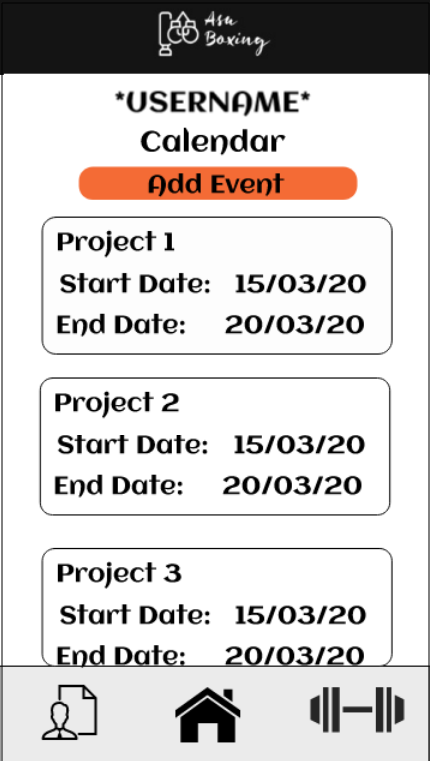
\includegraphics[width=0.25\textwidth]{images/profilePageBorder.png}
\caption{\label{fig:pComponent}Days}
\end{wrapfigure}




As can be seen in figure \ref{fig:pComponent} it firstly displays the Username and Calendar. This is for the reassurance and a quick simple explanation towards the user of what the component consists of.\\
As explained above this component is connected to the calendar plugin from the mobile device therefore we designed the applications to present the user with the already made events in his/her calendar.
We extract the following information from these events 
\begin{itemize}
    \item Name of the event
    \item The start date of the event
    \item The end date of the event
\end{itemize}
we output them to the user as displayed in figure \ref{fig:pComponent}.
This section is also designed to give the user an option to add an even for example a workout. The applicant can execute this with the $add-event$ button displayed underneath the user information.
This button connects to the calendar plugin and brings the applicant to the add section of the calendar application once the event is added user is back in  ASU Boxing with the newly created event present.

\section{Workout Component}

\begin{wrapfigure}{R}{0.3\textwidth}
\centering
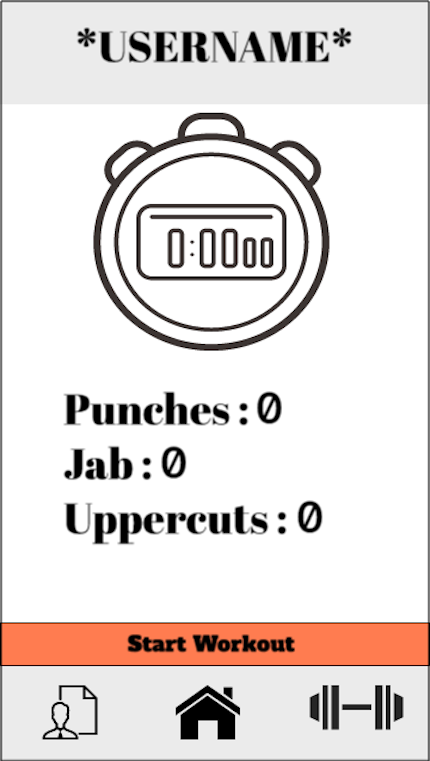
\includegraphics[width=0.25\textwidth]{images/workoutBorder.png}
\caption{\label{fig:isWComponent}Days}
\end{wrapfigure}




The workout component is loaded when the bottom right tab is pressed.\\
This component is designed to carry out and display to the user a lot of the applications functionality.\\
Figure \ref{fig:isWComponent}  shows this component, at the top the user name is displayed just as a way of connecting the application with the user therefore he/she can be assured that we have loaded in the correct user information.\\
Below the user name we have a timer for the specified workout time. The costumer has the ability to chose length of time themselves, the timer outputs the time selected and starts timing down when the button at the bottom of the screen $Start-Workout$ is selected. When the time is finished the application is designed to call the vibration plugin, ultimately when the workout is completed the phone should Vibrate.
The vibration is put in as a reminder to the user when the time has finished we designed this feature because we are well aware that when workouts are carried out applicants would concentrate more so on the workout itself than the application hence the vibration is a finish line for the workout.
\newpage
\begin{wrapfigure}{L}{0.3\textwidth}
\centering
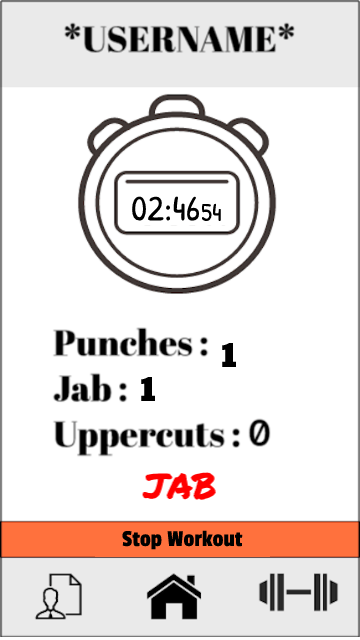
\includegraphics[width=0.25\textwidth]{images/workoutAfterPunch.png}
\caption{\label{fig:ipWComponent}Workout component during workout.}
\end{wrapfigure}
This part of the application is designed to count the number of punches and recorded display the information to the user. In the above image we see the component at its initial stage where the amount of punches are zero.
The start button will be connected to the accelerometer, gyroscope and the neural network. Working in conjunction they gather the three way axis information to determine if a punch is present, which punch it is and if its a valid punch.
Another feature in this part of the application is when a punch is thrown it is printed out to the screen as can be seen in figure  \ref{fig:ipWComponent} in red colour the name of the punch is printed to the user and both the number of punches as well as the number of the punch carried out are increased.






\begin{wrapfigure}{R}{0.3\textwidth}
\centering
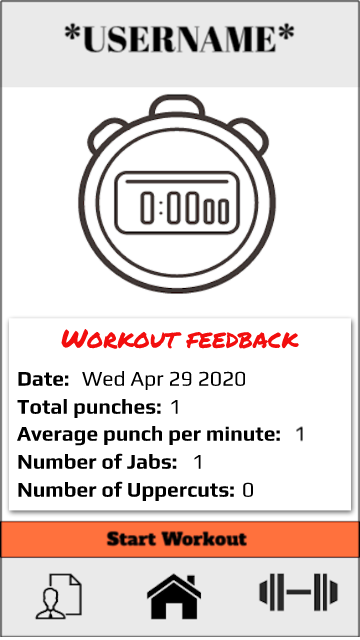
\includegraphics[width=0.25\textwidth]{images/afterWorkout.png}
\caption{\label{fig:ipWComponent}Workout component during workout.}
\end{wrapfigure}




The application has also the design that gives the user an option to to end a workout at anytime this can be done with the $Stop-Workout$ button shown in figure \ref{fig:ipWComponent}.
When the workout is finished or stopped the application gives out the results from the exercise.

Shown in figure \ref{fig:aWComponent} is the design of the results displayed out to the user the results will consist of 
\begin{itemize}
    \item Current Date 
    \item Total amount of punches
    \item Average amount of punches per minute
    \item Number of Jab punches
    \item Number of Uppercut punches
\end{itemize}
Workout feedback was designed to summarise the workout for the applicant also for the users to be able to analyse their performance and set goals for future workouts. 




\chapter{Conclusion}
This chapter will summarise the project in terms of the objectives of
the initial proposal and will discuss the findings and outcomes of the
project now it has concluded.
The project proposed the development of an ionic, angular, android application
with an AI punching detection system using Tensorflow, user details stored in Firebase an online
database and meals as well as workouts stored on a database in server on the cloud.

\section{Objectives \& Goals}
\begin{itemize}

\item Deploy a working application on to the official android store.\\
\textbf{PASS OR FAIL}
\item Design and Develop a user friendly application which will be easy to understand and use by any given person.\\
\textbf{PASS OR FAIL}
\item Find a way to integrate neural networks in conjunction with the angular environment and teach the machine learning part of the project to recognize persons hand movements.\\
\textbf{PASS OR FAIL}
\newpage
\item To work as a developing team, work as professionally as possible set objectives and complete them. Meet up on weekly basis with project development updates and discussions about the application.\\
\textbf{PASS OR FAIL} 
\item Connect the application and display the information from a self developed server with our own designed database of meals and workouts.\\
\textbf{PASS OR FAIL}
\item For the application to to have a valid log in and sign up connected to a database that stores the users information.\\
\textbf{PASS OR FAIL}
\item Allocate the work evenly and fairly between the three of us and set goals for each one of us.\\
\textbf{PASS OR FAIL}
\item Constantly testing the application will allow for error and bug detection detection as well as advance the development of this application. The application should be tested every time it is updated and documented on the results.\\
\textbf{PASS OR FAIL}  
\end{itemize}
\newpage
\section{Retrospective of the project}

We had found the ionic, angular and cordova documentation extremely useful and helpful. 
The documentation was easy to follow and very detailed in the description of the steps necessary to complete chosen tasks.
We used the documentations in the set up of the software connecting ionic cordova and angular but also in the testing and deploying of the application.\\
This project required certain plugins such as the device motion this was used for the accelerometer and we used the ionic documentation to install and use it as well as all the other plugins necessary.
Ionic documentation was very detailed giving us plenty of help in the development.

Using something like Firebase really gave us an opportunity to work on the rest of the application without having most of the back-end, we do have our own back-end server but we didn't want to have users personal information in case our application got compromise. Firebase was originally used for security and was really easy understand due the like well written documentation you can find online. I would highly recommend using Firebase to any developer that plans on starting a new application and isn't ready to handle all the back-end server issues. \\

Tensorflow is a really powerful tool for developing neural networks. This powerful tool is also easy to use and that's why we choose to use Keras with Tensorflow. There is a countless amount of documentation available online for developers to make a neural network for anything a developer desires to use it for. This really helped us get more accurate results for our punches, more specifically the upper-cut that the accelerometer had a issues properly calculating.\\

Learning about databases is quiet educational. It is very interesting how databases play their part whether it's within an application or a webpage. MySQL is a database software. It used "SQL" language to query the database. The combination of MySQL, WAMP Server and AWS is unique. In this project, one is depending on another. Amazon offers a brilliant hosting service which is called AWS (Amazon Web Services). Creating a virtual machine on Amazon and setting it up for this project was a brilliant moment to learn about the services provides to students from a great company like Amazon.\\
Wamp/Wamp Server is a software that allows us to use our computers as local servers, and "host" websites or applications on it. It was a very useful tool for us to check how our application would work on a dedicated server, especially for back-end aspects, like MySQL.
I would personally recommend using MySQL to any developer that wishes to start a new application and plans on using a back-end server. I feel with all the help out there given by experts, SQL is an easy and understanding language to pick up on.

\section{Future Improvements}
This section of the conclusion has the description of the possible future implementations that we have decided on. We feel these improvements would help this application move forward in the software industry gain popularity and improve the overall user exper\bodyience while not damaging the applications performance.\\

\textbf{Applications Improvements}\\
There are certain aspects of the application that that didn't quite come out as it was planned at the beginning and due to the project time frame certain features were not included.
The improvements in the application that we believe can bet made are as follows the punching detection system we would like to maximize Tensorflow's performance and connect it to the application and have the highest correct punch detection percentage as possible.\\
At the beginning we planned this application to have the option for multiple amount of exercises such as running, cycling and walking. This was not completed but we feel in the future this is very much possible by implementing certain plugins and connecting their data to the application.\\  


\textbf{Hardware Design}\\
From the beginning we knew that the application would be suitable for a mobile device but it was obvious another bit of hardware would give it the edge that is necessary to make it work in the real world.
At the moment the application is developed on the phone and its not ethical for a boxer to be holding the phone in his hand while practicing punching.

We planed many ideas for this implementation and when the time is right we would love to design and develop our own hardware with built in accelerometer and gyroscope.
This piece of hardware would connect to the application but also be inserted into a boxing glove possibly into the gloves strap this could allow the boxer to fight freely without noticing the hardware and at the same time receiving results back from the program.\\

\textbf{Boxing Environments}\\
Another future implementation for this application is exposing it to the boxing environment. When this application is completed and hardware is connected we would love to introduce the app to boxing, MMA and all other fighting clubs.
This would help us with with feedback from actual fighters and determine if there is any future in this application.\\

\textbf{iOS}\\
This application is currently developed for and Android device and for the Play store. In the near future we would love to widen the availability of the application across as many platforms as possible.
iOS devices and the iOS app store are as popular as the android environment therefore deploying the application for iOS could make significant difference to the applications popularity.

\chapter{Appendices}

\section{Instalation Guide}
\textbf{Github Repository link:} https://github.com/ArekMamala/FinalYearProject \\

Download and install Cordova, Angular and Ionic using the following
link:
\begin{itemize}
    \item \textbf{Cordova: } https://cordova.apache.org
    \item \textbf{Angular: } https://angular.io/guide/setup-local
    \item \textbf{Ionic: } https://ionicframework.com/getting-started\\
\end{itemize}

With all the frameworks and SDK's out of the way, we can begin setting up
the project files. 
Begin by cloning the GitHub repository, this can be done from the command line using the following command:
\begin{lstlisting}
    git clone https://github.com/ArekMamala/FinalYearProject
\end{lstlisting}{}

When the project is set up correctly plugins and platform's in the application will have to be added into the project and installed using the commands stated below.\\
\section{Plugins}
\textbf{Vibration}
\begin{lstlisting}
    ionic cordova plugin add cordova-plugin-vibration
    npm install @ionic-native/vibration
\end{lstlisting}

\textbf{Calendar}
\begin{lstlisting}
    ionic cordova plugin add cordova-plugin-calendar
    npm install @ionic-native/calendar
\end{lstlisting}


\textbf{Device Motion}
\begin{lstlisting}
    ionic cordova plugin add cordova-plugin-device-motion
    npm install @ionic-native/device-motion
\end{lstlisting}{}


\textbf{Device Gyroscope} cordova-plugin-gyroscope 0.1.4 "Device Gyroscope"
\begin{lstlisting}
    ionic cordova plugin add cordova-plugin-gyroscope
    npm install @ionic-native/gyroscope
\end{lstlisting}


\textbf{SQLite-Storage}
\begin{lstlisting}
    npm install mysql
    npm install cors
\end{lstlisting}


\textbf{Splash screen}
\begin{lstlisting}
    ionic cordova plugin add cordova-plugin-splashscreen
    npm install @ionic-native/splash-screen
\end{lstlisting}{}


\textbf{Firebase}   
\begin{lstlisting}
    npm install firebase --save
    npm install -g firebase-toolsso
\end{lstlisting}





unknown\\
cordova-plugin-compat 1.2.0 "Compat"

cordova-plugin-device 2.0.2 "Device"

cordova-plugin-ionic-keyboard 2.2.0 "cordova-plugin-ionic-keyboard"
cordova-plugin-ionic-webview 4.1.3 "cordova-plugin-ionic-webview"

cordova-plugin-screen-orientation 3.0.2 "Screen Orientation"

cordova-plugin-statusbar 2.4.2 "StatusBar"
cordova-plugin-whitelist 1.3.3 "Whitelist"

\section{Platforms}
The following platforms can be used for testing and running the application on your local device.\\
\textbf{Android}   
\begin{lstlisting}
    ionic cordova platform add android
\end{lstlisting}

\textbf{Browser}   
\begin{lstlisting}
    ionic cordova platform add browser
\end{lstlisting}

\section{Running Application}

\textbf{Android}   
When running on android the device used for testing must be connected to the computer and that device must be selected when running the below command.
\begin{lstlisting}
    ionic cordova run android
\end{lstlisting}

\textbf{Browser}   
When running on browser a link to test the application will be displayed after the following command is entered.
\begin{lstlisting}
    ionic cordova run browser
\end{lstlisting}


\subsection{Android with APK file}
The applications SDK files are located in the Github repository in the releases section of the project.
https://github.com/ArekMamala/FinalYearProject/releases\\

To deploy the SDK file of the application we use the following command
\begin{lstlisting}
    ionic cordova build android --prod 
\end{lstlisting}
This results in a creation of an SDK file in the file directory displayed.\\
The following SDK needs to be transferred into the testing device and installed.

Installing unknown applications on your android device can be challenging if you are not aware of the application security system in the android environment.
The following steps are necessary for android users to run the applications apk file.
\begin{itemize}
    \item \textbf{Menu} - move to the menu section of the device.
    \item \textbf{Settings} - move to the settings section of the device.
    \item Check \textbf{Unknown Sources} to allow your phone to install apps from sources other than the Google Play. Store.
\end{itemize}
More recent versions of Android deal with this situation a bit differently, instead of you doing all the work above when you install an APK for the first time you are prompted to allow your browser or file manager to carry out this process.\cite{apkFiles} 


\section{Application images}

\begin{figure}[h]
    \begin{center}
    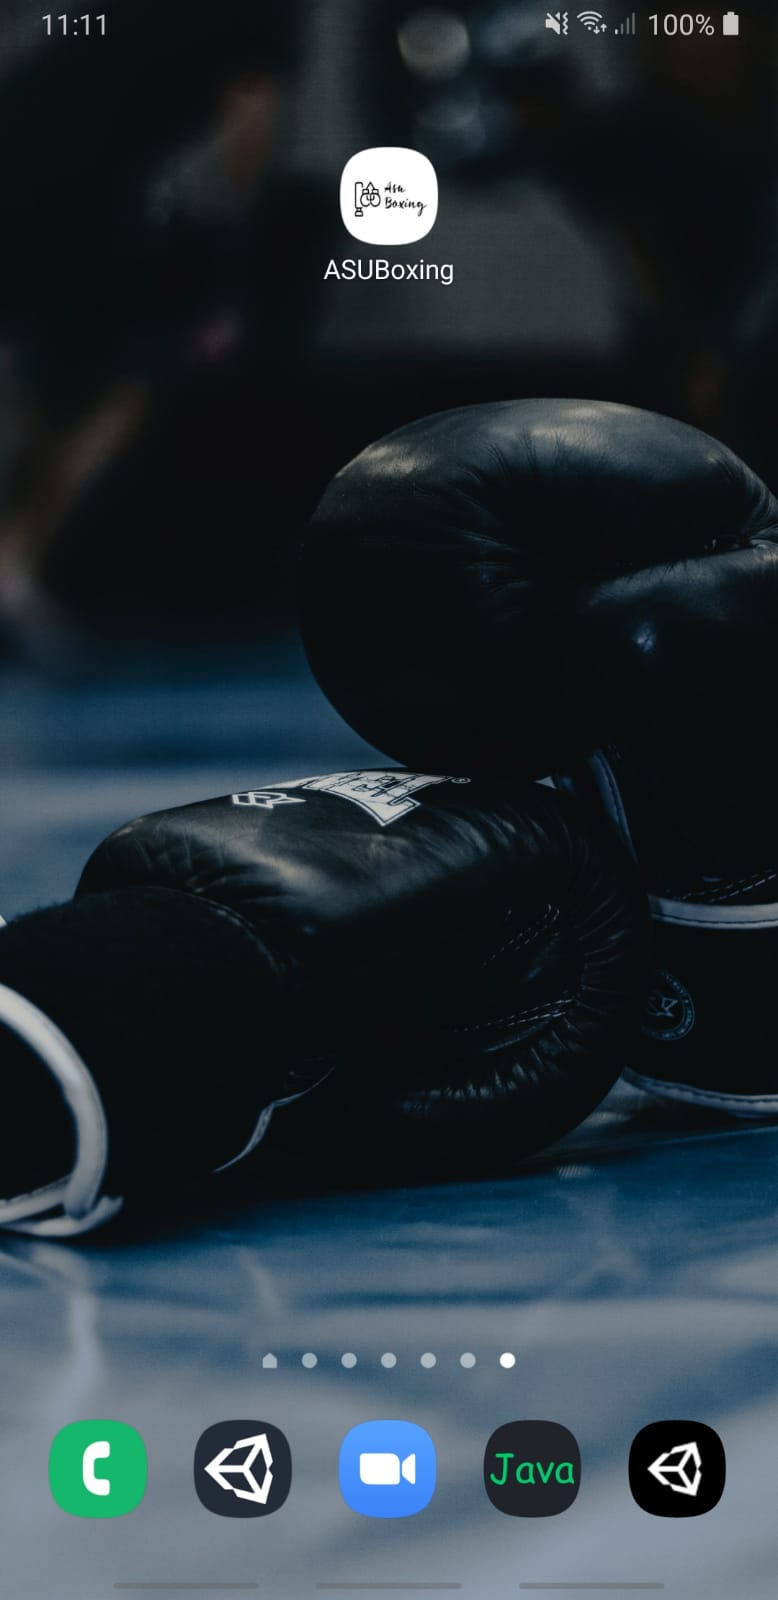
\includegraphics[scale=.1]{images/aplicationImages/application.jpeg}
    \hspace{1cm}
    
\includegraphics[scale=.1]{images/aplicationImages/splashScreen.jpeg}
    \caption{Application Installed and splash screen displayed}
    \label{fig:survey}
    \end{center}
\end{figure}
\begin{figure}[h]
    \begin{center}
    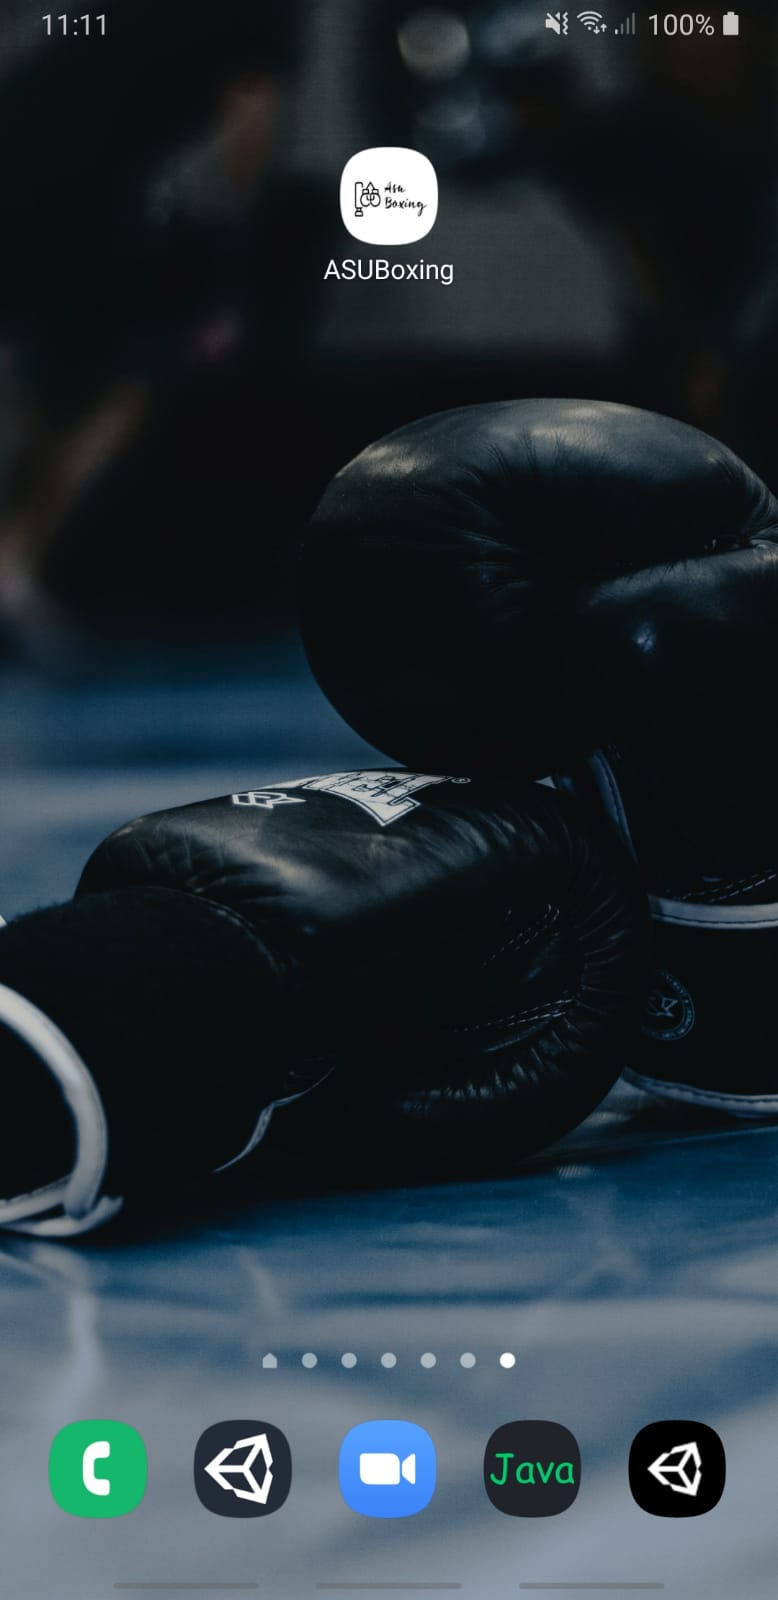
\includegraphics[scale=.1]{images/aplicationImages/application.jpeg}
    \hspace{1cm}
    
\includegraphics[scale=.1]{images/aplicationImages/splashScreen.jpeg}
    \caption{Application Installed and splash screen displayed}
    \label{fig:survey}
    \end{center}
\end{figure}







% references section
\bibliographystyle{plain}
\bibliography{refs} % 


\end{document}
